\documentclass[10pt,a4paper,twoside]{report}

%LOAD PACKAGES
\usepackage[T1]{fontenc}
\usepackage[italian,english]{babel}
\usepackage{hyperref}
\addto\extrasenglish{%
	\def\chapterautorefname{Chapter}}
\addto\extrasenglish{%
	\def\subsectionautorefname{section}}
\usepackage{graphicx}
\usepackage{rotating}
\usepackage{tabularx}
\usepackage{amsmath}
\usepackage{listings}
\usepackage[printonlyused,withpage]{acronym}
\usepackage{frontespizio}
\usepackage{imakeidx}
\usepackage{comment}
\usepackage[table,usenames,dvipsnames]{xcolor}
\usepackage{xcolor}
\usepackage{setspace}
\usepackage{titlesec}
\usepackage{chemformula}
\usepackage{varioref}
\usepackage{subfigure}
\usepackage{alphalph}
\usepackage{siunitx}
\usepackage{multirow}
\usepackage{array}
\usepackage[nottoc]{tocbibind}
\usepackage[a4paper]{geometry}
\usepackage{pdfpages}


%\usepackage{url}
%\usepackage{listings}
%\usepackage[toc]{appendix}

%[display]

\titleformat{\chapter}%
  {\normalfont\bfseries\huge}{\thechapter.}{10pt}{}

% Cartelle da cui recuperare le immagini
\graphicspath{{immagini/}, {grafici/}, {first/}, {second/}, {third/},{fourth/}, {fifth/}}

%Indice
%\makeindex

%Indice dei contenuti
\hypersetup{
    colorlinks = false,
    allbordercolors = {white}
}

%Numerazione subsubsection
\setcounter{tocdepth}{3}
\setcounter{secnumdepth}{3}


%COMMAND TO INCREASE POSSIBLE LABELS IN CAPTION
\renewcommand*{\thesubfigure}{(\alphalph{\value{subfigure}})}

%COMMAND TO DEFINE NEW TYPE OF COLUMN(per andare a capo e centrare il testo)
\newcolumntype{C}[1]{>{\centering\let\newline\\\arraybackslash\hspace{0pt}}m{#1}}

%VARIOREF
\vrefwarning






%------------------------------------
%		INFO
%------------------------------------

%\title{Studio di rivelatori a pixel monolitici CMOS per l'upgrade dell'esperimento Belle II}
%\author{Mara Stefania Calò}
%\date{9 Novembre 2022}
%\newcommand{\institution}{Università di Pisa}
%\newcommand{\department}{Dipartimento di Fisica}

%--------------------------------------
%		TITLE
%--------------------------------------


\begin{document}

%Contenuti
\doublespacing
\tableofcontents
\singlespacing


\begin{comment}
\begin{frontespizio}
\Universita{Pisa}
\Logo[scale=.1]{logo}
\Dipartimento{Fisica}
\Corso{Fisica delle Interazioni Fondamentali}
\Titolo{Studio di rivelatori a pixel monolitici CMOS per l'upgrade dell'esperimento Belle II}
\Candidato{Mara Stefania Calo'}
\Relatore{prof. Francesco Forti}
\Annoaccademico{2022.2023}
\end{frontespizio}
\end{comment}

\newpage

% --------------------------------------------
%		ABSTRACT 
%---------------------------------------------
\section*{Abstract}

\begin{comment}
Belle II è un esperimento di fisica delle particelle situato a Tsukuba, in Giappone, nel laboratorio (di) KEK (100 km da Tokyo). E' una flavor-factory di seconda generazione che opera alla frontiera dell'intensità, detenendo il record mondiale di maggiore luminosità. L'acceleratore SuperKEKB è un collider di fasci $e^{+}$ $e^{-}$ con energie asimmetriche e piccate alla risonanza $\Upsilon$(4S). Auspica a raccogliere un set di dati fino a 50 $ab^{-1}$ (x50 Belle dataset, x100 BaBar dataset) per studiare la violazione di CP nei mesoni B e ricerca nuova fisica oltre il Modello Standard.
\end{comment}


% --------------------------------------------
%		CAPITOLO 1 
%---------------------------------------------
\input{first\_chapter}


% --------------------------------------------
%		CAPITOLO 2 
%---------------------------------------------
\input{second\_chapter}


% --------------------------------------------
%		CAPITOLO 3 
%---------------------------------------------
\input{third\_chapter}


% --------------------------------------------
%		CAPITOLO 4
%---------------------------------------------
% --------------------------------------------
%		CAPITOLO 3 
%---------------------------------------------
\chapter{VTX detector} \label{ch:VTX}


This chapter focuses on one of the four proposals for the vertex detector upgrade of Belle II, that is VTX. After a brief reference to the reasons behind the vertex detector upgrade, we will go trough VTX concept and layout, designed with a new geometry with respect VXD and also with a different mechanical structure and new pixel sensors (OBELIX), needed to fulfill the new requirements dictated by new environment conditions. Moreover all ongoing studies are supported by continual tests and simulations that we will also take a look at.


%---------------------------------------------
%			3.1
%---------------------------------------------
\section{VTX Layout and mechanical structure}

In~\autoref{sec:nano_beam} we have introduced in a few words the concept of the \textit{nano-beam} scheme, which could allow to achieve the new target of instantaneous luminosity. This new strategy requires a strong focusing of the beams in particular at the IP, resulting in a large amount of beam induced background and as consequence in a higher dose of radiation in the innermost detector layers. Therefore they have to be robust enough to keep good performance against these new hard conditions.
Furthermore to be able to increase the luminosity, SuperKEKB might have to consider an improvement of the final focusing magnets and so a potentially re-design of the interaction region, including the detector but independently of its hit rates and radiation hardness issues.\\

\begin{figure}[h!]
\centering
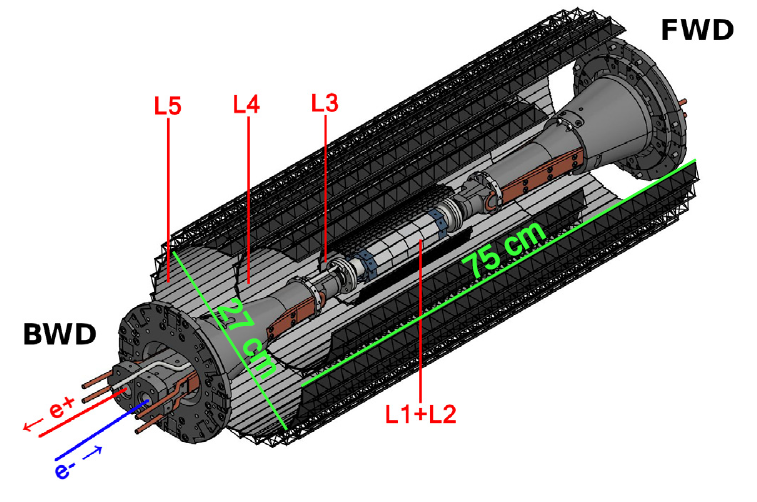
\includegraphics[scale=.6]{VTX_layers}
\caption{Concept of VTX layout with 5 barrel layers, filling the current VXD volume.}
\label{fig:VTX_layers}
\end{figure}


VTX project aims to replace the all VXD with a fully pixelated detector based on Depleted Monolithic Active Pixel Sensors (DMAPS) arranged on five layers at different distance from the beam pipe (\autoref{fig:VTX_layers}). Actually the radii and the number of the layers are currently subject to several  studies and simulations, in order to achieve an optimized arrangement. 
For now two layers are planned in the innermost part (\textit{i}VTX) and three in the outermost (\textit{o}VTX). The active lenght of the ladders is expected to vary from 12 to 70 cm to cover the required acceptance of $17^{\circ} < \theta < 150^{\circ}$.\\
As already discussed for the other upgrade proposals, it is important to try to reduce the material budget, in order to minimize the multiple Coulomb scattering which particularly affects the very soft particles produced in Belle II collisions. By using a single sensor type, it is expected a reduction of the overall material budget up to 2\% of radiation lenght, against the present 3\% of VXD, which uses two different sensors such as pixels and strips.


\subsection{iVTX}

The \textbf{\textit{internal}VTX} consists of the first two detector layers devised togheter with a self-supported air-cooled all-silicon ladder concept, where four contiguous sensors are diced out of a wafer, thinned and interconnected with post-processed redistribution layers. They are designed to be at 14 and 22 mm respectively from the beam pipe, and target an individual material budget of about 0.1\% radiation lenght. 
This is actually achivable because the overall surface of these layers is moderate, below 400 $cm^{2}$, as well as the sensor power dissipation is expected to be low and the connections needed for the operation to be a few. Precisely for these reasons, air cooling could be a workable system to avoid overheating.


\begin{figure}[h!]
\centering
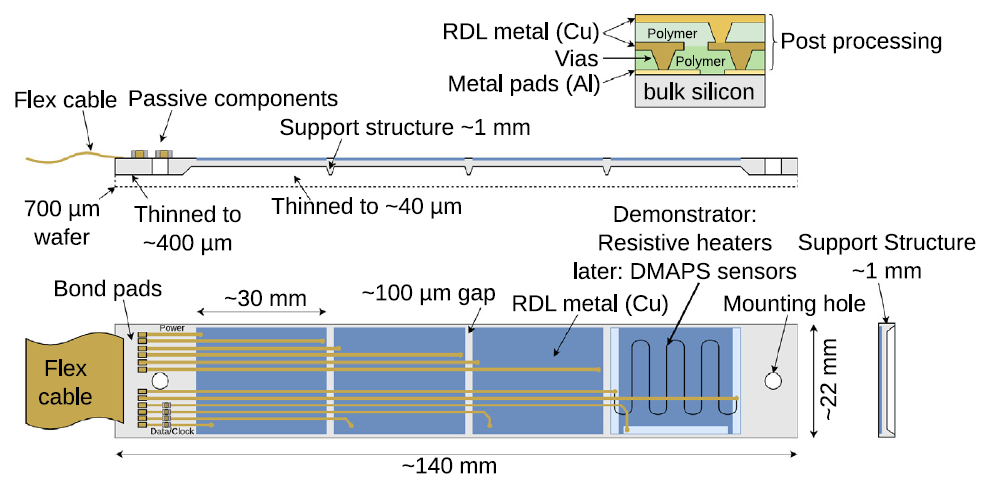
\includegraphics[scale=.65]{iVTX}
\caption{Sketch of the all-silicon ladder concept of the iVTX. Four dummy sensors are shown in blue on the silicon support in grey. The yellowish lines instead, indicate power and data transmission lines. Power is delivered to the ladder by a flex cable, which also transmits data to and from the chips in the final one.}
\label{fig:iVTX}
\end{figure}

The ladder has to be equipped with four of the aforementioned OBELIX chips and thinned to 50 $\mu$m except in some border regions, where a few hundreds of $\mu$m are necessary to ensure mechanical stability. 
In order to interconnect the sensors along the ladder and provide a unique connector at the backward end, during the post-processing metal strips are etched on the redistribution layer (RDL). The latter has the main purpose to route power and data via impedence-controlled transmission lines to a flex cable, added at the end of the ladder.
After the RDL processing, the backside of the ladder has to be thinned in accordance with what was previously mentioned. Mounting holes will be added via laser-cutting.


In~\autoref{fig:iVTX} is displayed a sketch of the iVTX demonstrator ladder (currently under production), 140 mm long and 22 mm wide (grey). Instead of the actual sensors, it is equipped with four dummy chips with a lenght of about 30 mm (blue), which are used as resistors to mimic the estimated heat load in order to test the air cooling system and more generally to characterized the electrical, mechanical and thermal performance of the ladder.
A redistribution layer for power and data is also added to the demonstrator, in order to connect the chips with a flex cable at the end of the ladder (yellowish lines). In addition the wafer is thinned to 400 $\mu$m and the sensitive areas down to 40 $\mu$m with the purpose to test the mechanical integrity of the whole structure.

\begin{description}
\item \textbf{Research and Development (R\&D)}
\end{description}

The R\&D is ongoing and the full-silicon ladder concept is currently being assessed with industrial partners. First thinned ladders have been produced and characterised with different thickness and geometry.

Furthermore several tests are focused on evaluating power delivery efficiency, the quality of the signals which travel through the ladder and also the process used to fully assembly it. 
In~\autoref{fig:iVTX_eye} are shown eye diagrams from simulation with a transfer rate of 640 Mbps, which may imply that 320 Mbps of data rate will be possible.

\begin{figure}[h!]
\centering
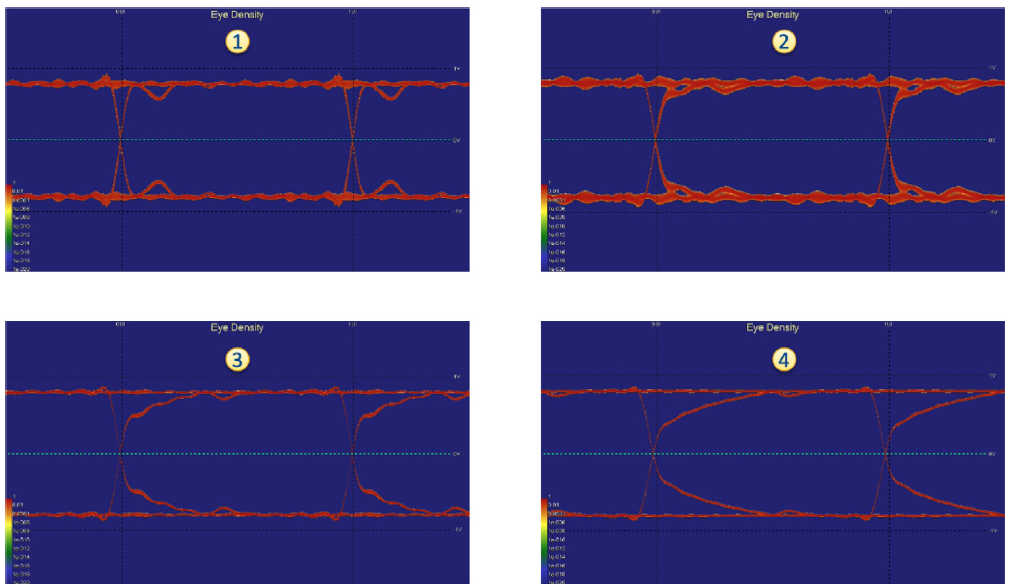
\includegraphics[scale=.7]{iVTX_eye}
\caption{Eye diagrams of the iVTX data transmission lines at four different locations on the ladder.}
\label{fig:iVTX_eye}
\end{figure}

Moreover it has been demonstrated that air at the temperature of $15^{\circ}$ and flowing with a speed of 10 m/s succeeds to cool a single inner module, assuming power is uniformly dissipated on the sensor surface. The maximum temperature reached is $20^{\circ}$C. 

Through very first estimates it is expected that an equivalent section of 6 tubes with 10 mm of diameter is necessary to expel the heat from the inner layers, roughly equal to 65 W. So it is essential to design a mechanical structure which provides for the space needed to the tubes in order to bring the air at the IP and also compatible with the new interaction region.


\subsection{oVTX} \label{sec:oVTX}

The \textbf{\textit{outer}VTX} consists of three layers respectively at radii of 39 or 69, 89 and 140 mm from the beam pipe and because of the larger distance required to cover the acceptance, they are not self-support. They follow a more traditional approach, strongly inspired by the design developed for the ALICE ITS2. Each ladder is water cooled and made of a light carbon fiber support structure, called \textbf{\textit{truss}}, which provides the mechanical integrity. Its structural design is shown in~\autoref{fig:oVTX} : 70 cm long and 5.8 g of weight, it is able to support more than 40 sensors in two rows next to each other with a small overlap, earning a material budget of 0.3\% $X_{0}$ for the first two layers and 0.8\%$X_{0}$  for the outermost one.

\begin{figure}[h!]
\centering
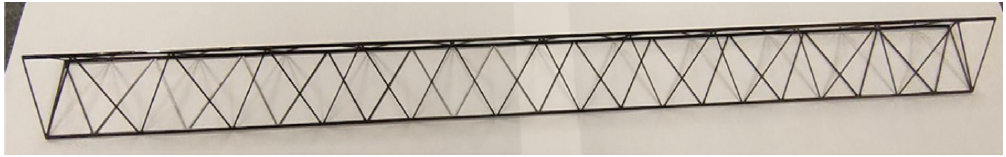
\includegraphics[scale=.7]{oVTX}
\caption{Prototype of the layer 5, called \textit{truss}, which is the longest, made from thin carbon fibre structures.}
\label{fig:oVTX}
\end{figure}


For the cooling of the ladder a cold-plate concept is under development (\autoref{fig:oVTX_coldplate}), on which the sensors are glued and that in turn is installed on the \textit{truss}. For each row there is a polymide cooling tube that runs over all the sensors and turns back at the other end, so that the heated coolant leaves on the same side. Then two flex print cables connect the two halves of the ladder to the connector.


\begin{figure}[h!]
\centering
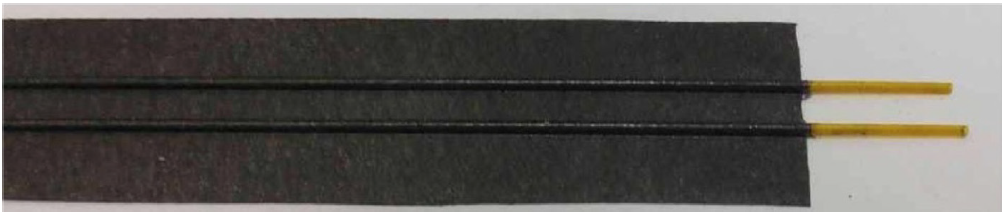
\includegraphics[scale=.7]{coldplate}
\caption{A prototype of the cold-plate for cooling. One coolant tube(golden) is connected to the cold plate(black) and turns 180° on the other end (not shown) so that the coolant flows in both directions and thus leaves on the same side it starts.}
\label{fig:oVTX_coldplate}
\end{figure}

For layer 3 instead, only one flex print cable in the backward side is considered, in order to leave more space in the forward for other possible services and accelerator components. As mentioned above, for the third layer two different solutions are under study: at radius of 39 mm e 69 mm respectively. 
In~\autoref{fig:ladders} are displayed schematic examples of some hypotheses. 

\begin{figure}[h!]
\centering
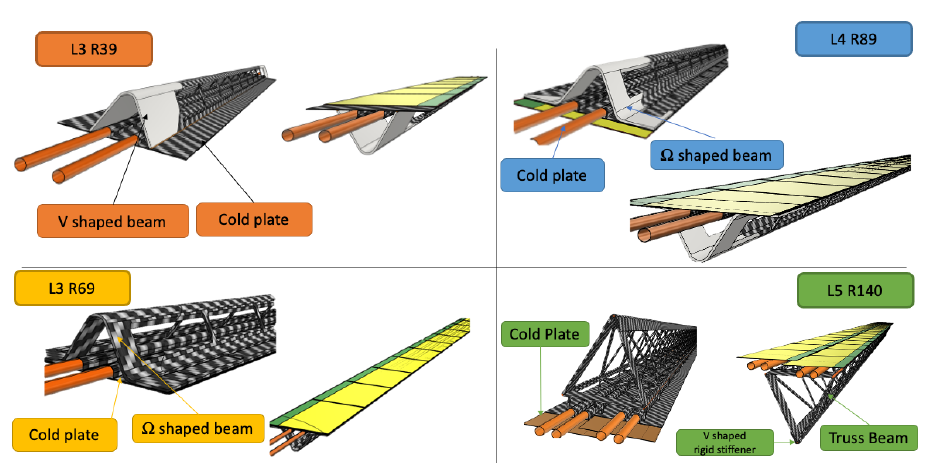
\includegraphics[scale=.7]{ladders}
\caption{Schematic view of possibile solutions for the three outermost layers.}
\label{fig:ladders}
\end{figure}


In~\autoref{fig:oVTX_5} are shown the several substructures described before, that shape a ladder of the outermost layer 5. From bottom to top come in succession the carbon fibre structure, two cold-plates for the two neighbouring sensor rows (indicated as ''Chips'', in grey) and the flex cables for power and data transmission (green). 


\begin{figure}[h!]
\centering
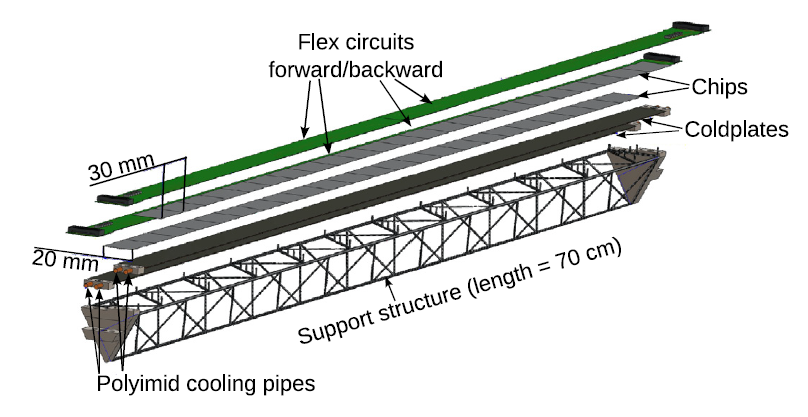
\includegraphics[scale=.7]{oVTX_5}
\caption{An exploding drawing of a fully assembled layer 5 ladder.}
\label{fig:oVTX_5}
\end{figure}

\begin{description}
\item \textbf{Research and Development}
\end{description}

The carbon fiber support structure and flex cable have been designed and fabricated for the last ladder, which is also the longest. Services for the last two ladders, like electrical connections and cooling, can be provided both on forward and backward sides.
A Multiline Power Bus has been realized in order to power each OBELIX chip along the ladder by a dedicated VDD and GND pair. \\

After the assembly described in the previous, first thermo-mechanical tests have been performed and they show that the first resonance frequency is at 200 Hz, which is safely far from the one of the typical earthquakes in Japan, and also that the thermal properties are good.\\

Trying to reduce as much as possible the material budget, the transmission lines and the flex cables have to be as thin as possible, but they also have to ensure safe data transmission. Trace widths are trimmed to fulfill the same maximum voltage drop requirement (200 mV) for all the chips.

For this reason, the outermost ladders (70 cm long) are equipped with two flex cables, one from each side of the \textit{truss}. In~\autoref{fig:oVTX_eye} the resulting eye diagram from testing the signal integrity of one of the 35 cm long transmission lines for data transmission rate of 500 Mbps. This result demonstrates that the bandwidth is large enough to allow more then needed 160 Mbps for data transmission.


\begin{figure}[h!]
\centering
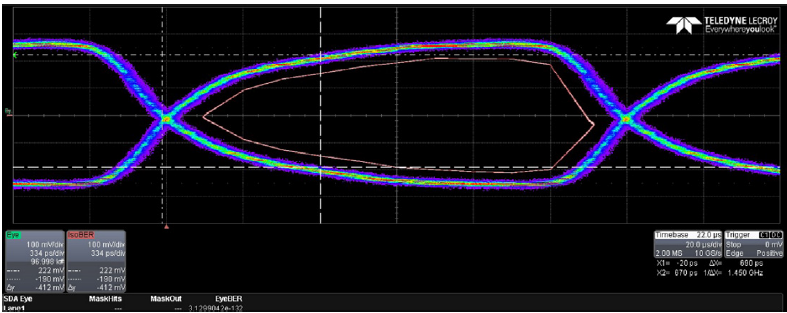
\includegraphics[scale=.8]{oVTX_eye}
\caption{Eye diagram for the oVTX transmission line signal integrity of the layer 5 flex cable.}
\label{fig:oVTX_eye}
\end{figure}


In addition, thermal tests have been performed for the last layer prototypes using kapton heaters to emulate the power dissipation of the chips. The coolant (demineralized water) has been set to a temperature of $10^{\circ}$ at the beginning, the environment at $20^{\circ}$ with a negative pressure of 0.2 bar. Results have been demonstrated that for three different configurations of the flow (such as monodirectional, bi-directional and with an U-turn at one end) the average temperature stands at $24^{\circ}$ with a maximum gradient of $\Delta T \approx 4^{\circ}$ along the full lenght of the ladder. 

All these investigations validate the design of the longest ladder, which is indeed the most challenging, and therefore the possibility to operate the chips safely.


\subsection{Thermomechanics and data transmission}

The proposed VTX detector intends to employ the same sensor type for all the layers in order to use a unique control and power supply system. It is expected to operate at room temperature and for what we have seen in the previous, the smaller cross section of data cables, the usage of optical fibers and the less complex cooling system might allow a considerable reduction of services with respect to the current VXD. This allows more room for maneuver in the design of the new IR, needed for ramping up the instantaneous luminosity in the future.

As consequence also the design of the mechanical support system, data cables and acquisition system required could be more simple and in particular, the standard PCIe40 acquisition boards used in Belle II match well the data throughput requirement.

%---------------------------------------------
%			3.2
%---------------------------------------------
\section{Performance simulation}


As we have seen in~\autoref{ch:upgrade}, increasing the luminosity implicates higher level of machine related background and so larger doses of radiation, expecially in the inner layers of the whole detector. 
For these reasons a lot of simulations and studies are focusing on ensuring that the main physics goals of the experiment will be achieved despite the more severe working conditions. 

The VTX upgrade program wich provides for a new silicon vertex detector with high granularity in both space and time, could bring significant improvements in tracking efficiency expecially at low momentum, in the impact parameter resolution and in the robustness against backgrounds. Moreover, better vertexing performance entails not only improved time-dependent analyses of B and D mesons, but also an enhanced capability to distinguish among different decay topologies.


\subsection{Potential VTX geometries}

As we have already mentioned in the description of the oVTX layout (\autoref{sec:oVTX}), two different VTX geometries are currently under study, which differ only in the position of the third layer (\autoref{fig:ladders}).  

The \textit{\textbf{nominal}} geometry is expected to maximize the track impact parameter resolution and it places the third layer at 39 mm from the IP.
The \textit{\textbf{alternative}} geometry instead, aims to improve the $K_{S}^{0}$ reconstruction efficiency and the third layer is located at 69 mm from the IP.\\

Several simulations and investigations are ongoing and they are comparing performance of these two different layouts with that of the current Belle II detector (utilizing a full Geant4 simulation of the detector in the study of specific decay modes of interest). Moreover, the different machine background predictions are also examined in order to consider all effects and correlations. 

\subsection{Tracking efficiency at low momentum and impact parameter resolution}

Tracking efficiency at low momentum is one of the areas where the VTX upgrade scenarios show more promising results, particularly for the \textit{soft pions} originated from the decays of $D^{*\pm}$ mesons.

Studies are based on the reconstruction of the decay chain $B^{0} \rightarrow D^{*-}l^{+}\nu$, with $D^{*-} \rightarrow \bar{D}^{0} \pi^{-}_{soft}$ and $\bar{D}^{0} \rightarrow K^{+} \pi^{-}$ or $K^{+} \pi^{-} \pi^{+} \pi^{-}$. All background scenarios metioned in~\autoref{sec:bkg_predictions} are considered in the evaluation of the \textit{nominal} VTX performance and they are compared with the nominal Belle II geometry in the intermediate (\textbf{v2}) background hypothesis. In~\autoref{tab:simulation_low_mom} is shown what has been obtained.

\begin{comment}
\begin{table}[htbp]
 \caption{Reconstruction efficiency and purity for the the decay chain $B^{0} \rightarrow D^{*-}l^{+}\nu$, with $D^{*-} \rightarrow \bar{D}^{0} \pi^{-}_{soft}$ and $\bar{D}^{0} \rightarrow K^{+} \pi^{-}$, for the nominal Belle II detector at the intermediate background conditions (\textbf{v2}) and the nominal configuration of VTX in all three background scenarios.}
\label{tab:simulation_low_mom}
  \begin{center}
    \begin{tabular}{l|c|c|c|c}
      \hline\hline
      & Belle II (v2) & VTX (v1) & VTX (v2) & VTX (v3) \\
      \hline\hline
      Generated events & 32533 & 32559 & 32559 & 30255 \\
      \hline
      Correctly reconstructed signal & 10059 & 16913 & 16848 & 15583 \\
      \hline
      Combinatorial & 28495 & 51375 & 51826 & 47527 \\
      \hline\hline
      Efficiency & 30.9\% & 51.9\% & 51.7\% & 51.5\% \\
      \hline
      Purity & 26.1\% & 24.8\% & 24.5\% & 24.7\% \\
      \hline\hline
    \end{tabular}
  \end{center}
\end{table}
\end{comment}


\begin{table}[h!]
\centering
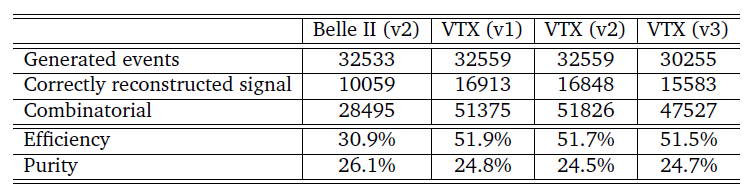
\includegraphics[scale=.9]{simulation_low_mom}
\caption{Reconstruction efficiency and purity for the the decay chain $B^{0} \rightarrow D^{*-}l^{+}\nu$, with $D^{*-} \rightarrow \bar{D}^{0} \pi^{-}_{soft}$ and $\bar{D}^{0} \rightarrow K^{+} \pi^{-}$, for the nominal Belle II detector at the intermediate background conditions (\textbf{v2}) and the nominal configuration of VTX in all three background scenarios.}
\label{tab:simulation_low_mom}
\end{table}

We can see that the VTX reconstruction efficiency\footnote{Efficiency is defined as the ration between the number of correctly reconstructed signal events and the total number of candidates.}  in all three background hypotheses, results to be improved of almost a factor 1.7 with respect to the nominal Belle II, with comparable purity\footnote{In a few words, the probability that a correctly reconstructed signal  is a ''signal event''.} . Moreover efficiency remains practically stable in all background conditions, even in the most severe one.

This enhancement in tracking efficiency relies in particular on improved tracking efficiency for the $\pi_{soft}^{-}$ mesons, as we can see in~\autoref{fig:simulation_soft_pi}.


\begin{figure}[h!]
\centering
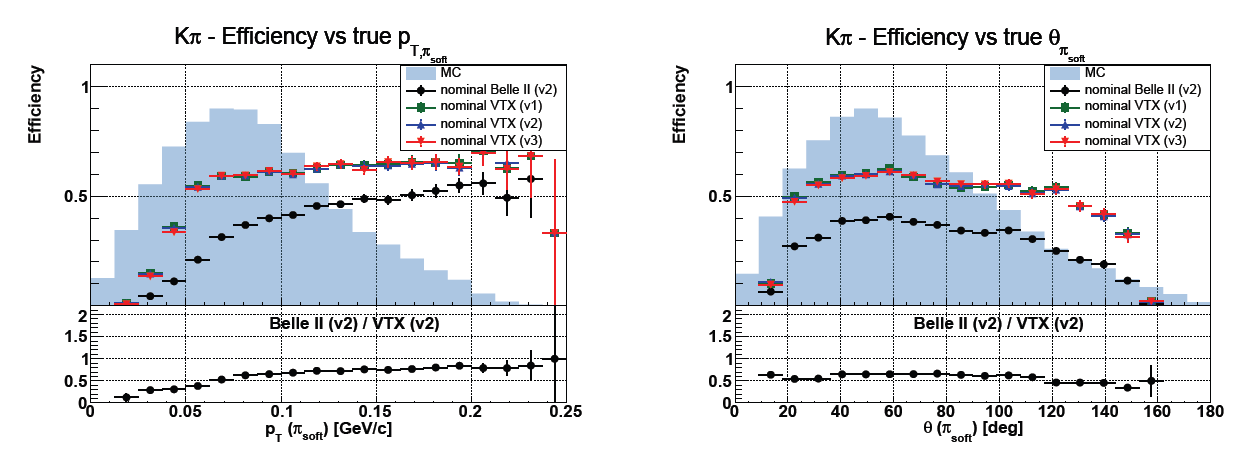
\includegraphics[scale=.53]{simulation_soft_pi}
\caption{Reconstruction efficiency of $B^{0} \rightarrow D^{*-}l^{+}\nu$ as a function of the transverse momentum of the $\pi_{soft}^{-}$ (from  $D^{*-} \rightarrow \bar{D}^{0} \pi^{-}_{soft}$) in the plot on the left and of the polar angle of the $\pi_{soft}^{-}$ on the right. 
The shaded blue histograms represents the momentum spectrum of the  $\pi_{soft}^{-}$.
The nominal Belle II geometry efficiency in the intermediate background scenario (\textbf{v2}) is represents by black dots and it is compared with the nominal VTX configuration in the optimistic (\textbf{v1}, green squares), medium (\textbf{v2}, blue upward pointing triangles) and pessimistic (\textbf{v3}, red downward
pointing triangles) background hypotheses. The bottom plots show the ration between nominal Belle II and nominal VTX in the \textbf{v2} background scenario.}
\label{fig:simulation_soft_pi}
\end{figure}

For all scenarios with nominal VTX, there is a powerful improvement for transverse momenta below 0.05 GeV/c, with respect to the nominal Belle II. Only for $p_{T}$ greater than 0.2 GeV/c the reconstruction efficiency of Belle II approach those of the VTX.\\

For $p_{T}$ higher than 0.3 GeV/c instead, the momentum resolution is dominated by the CDC and there is not a significant enhancement in track momentum resolution considering the preceding example.

\subsection{Vertexing resolution}

Studies on vertexing performance have been conducted using samples of one million $B^{0} \rightarrow J/\psi K_{S}^{0}$ events generated and reconstructed with all the aforementioned combinations.
The distributions of the decay vertex resolution $\sigma_{z}$ (i.e. the width of the distribution obtained considering the differences between the measured and the true simulated positions) along the \textit{z} axis of the B decay signal are shown in~\autoref{fig:simulation_vertex} .

\begin{figure}[h!]
\centering
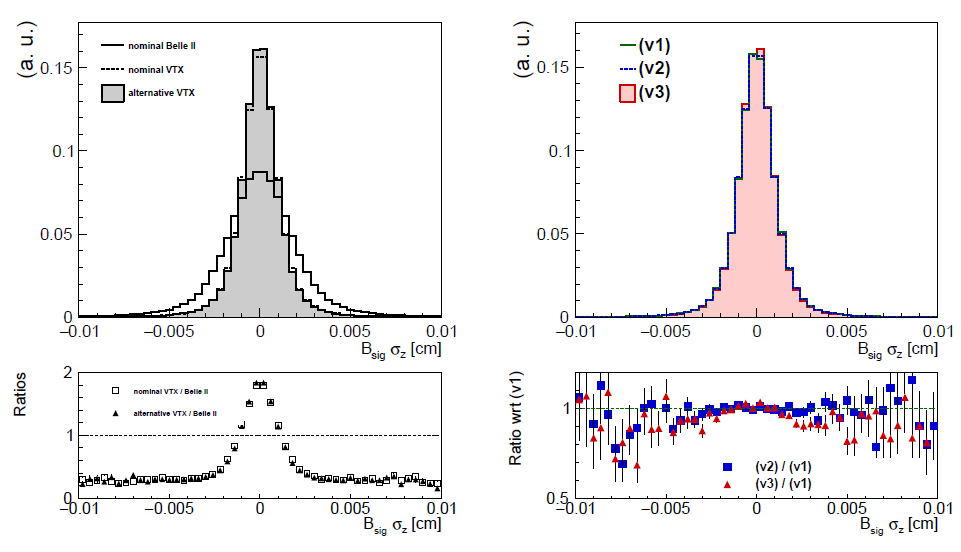
\includegraphics[scale=.65]{simulation_vertex}
\caption{On the left: comparison of the B decay vertex resolution along the \textit{z} axis in $B^{0} \rightarrow J/\psi K_{S}^{0}$ events for the nominal Belle II (solid line), nominal VTX (dotted line) and alternative VTX geometry (filled grey histogram). The bottom plot shows the ratio between the VTX geometries (empty squares the nominal one and filled triangles the alternative) and nominal Belle II. \\
On the right:  B decay vertex resolution along the \textit{z} axis for the nominal VTX geometry in the three background scenarios: optimistic \textbf{v1} (green solid line), intermediate \textbf{v2} (blue dotted line) and pessimistic \textbf{v3} (red filled histogram). The bottom plot represents the ratio between the two higher background scenarios and the optimistic one.}
\label{fig:simulation_vertex}
\end{figure}

In~\autoref{tab:simulation_vertex_table} a summary of the results that shows that the new geometries achieve a better resolution on the B decay vertex of about 35\% on average and they also do not suffer of any significant degradation as the background conditions varies, unlike the nominal Belle II configuration.

\begin{table}[htbp]
  \begin{center}
    \begin{tabular}{l|c|c|c}
      \hline\hline
      $B_{sig}$ $z$ vertex resolution ($\mu$m) & Bkg (v1) & Bkg (v2) & Bkg (v3) \\
      \hline\hline
      Belle II & 21.9 & 23.0 & 24.9 \\
      \hline
      Nominal VTX & 14.5 & 14.4 & 14.1 \\
      \hline
      Alternative VTX & 14.4 & 14.3 & 14.0 \\
      \hline\hline
    \end{tabular}
  \end{center}
\caption{$B_{sig}$ vertex resolution along the \textit{z} axis for the three detector layouts and the three background scenarios.}
\label{tab:simulation_vertex_table}
\end{table}

\begin{comment}
\begin{table}[h!]
\centering
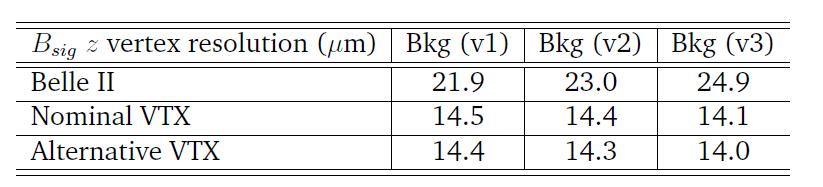
\includegraphics[scale=.8]{simulation_vertex_table}
\caption{$B_{sig}$ vertex resolution along the \textit{z} axis for the three detector layouts and the three background scenarios.}
\label{tab:simulation_vertex_table}
\end{table}
\end{comment}

The VTX geometries have been demonstrated to achieve better performance also for the vertexing resolution along the \textit{x} and \textit{y} axes. Also in these directions they turn out to be almost insensitive to the different levels of background.\\

Similar studies for the $K_{S}^{0}$ decay vertex resolution are displayed in~\autoref{fig:simulation_vertex_K} and in the same way, the upgraded geometries reach a better vertexing resolution with respect to the nominal Belle II detector without any sginifcant degradation as the backgrounds increase.
It is important to notice that in the right plot there is a spurious effect that cause an apparent improvement of performance in the worst case scenario among those considered. This is due to the loss of reconstruction efficiency for candidates with large flight distance (thus affected by poorer vertex resolution).

\begin{figure}[h!]
\centering
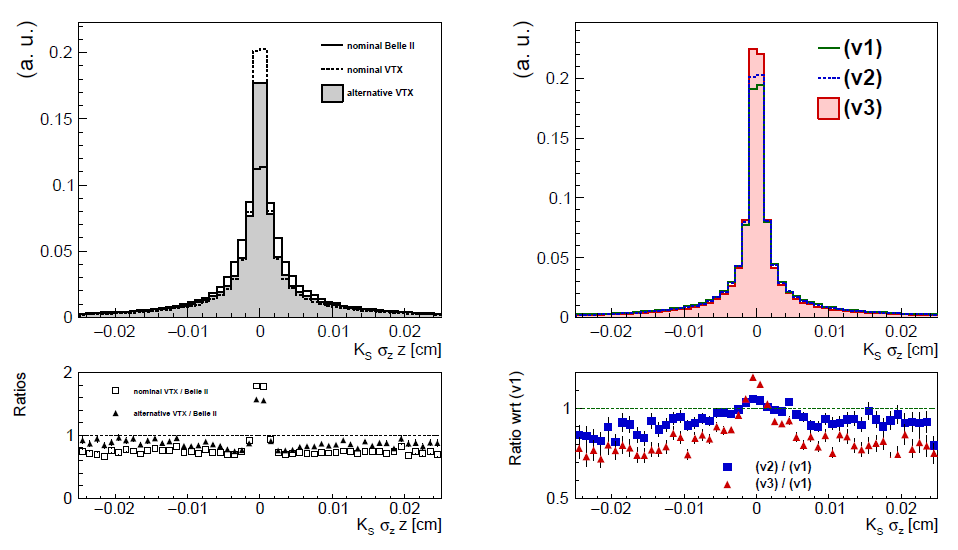
\includegraphics[scale=.65]{simulation_vertex_K}
\caption{On the left: comparison of the $K_{S}^{0}$ decay vertex resolution along the \textit{z} axis in $B^{0} \rightarrow J/\psi K_{S}^{0}$ events for the nominal Belle II (solid line), nominal VTX (dotted line) and alternative VTX (filled grey histogram). The bottom plot shows the ratio between the VTX geometries (empty squares for the nominal and filled triangles for the alternative) and nominal Belle II detector. 
On the right: $K_{S}^{0}$ decay vertex resolution along the \textit{z} axis for the nominal VTX in the three background scenarios: optimistic \textbf{v1} (green solid line), intermediate \textbf{v2} (blue dotted line) and pessimistic \textbf{v3} (red filled histogram). The bottom plot represents the ratio between the two higher background scenarios and the optimistic one.}
\label{fig:simulation_vertex_K}
\end{figure}


%---------------------------------------------
%			3.3
%---------------------------------------------
\section{OBELIX chip design}

The VTX detector is designed with a single type sensor taylored to the specific needs of Belle II, called OBELIX (Optimized BELle II pIXel sensor) and currently under development, based on fast and high granular Depleted Monolithic Active Pixel Sensor (DMAPS). This new sensor design comes from an evolution of TJ-Monopix 2, whose characterization is the main topic of this thesis, and which will be discussed in~\autoref{ch:TJ2}. Both of them are fabricated in a modified TowerJazz Semiconductor 180 $\mu$m CMOS process, that matches particularly well the Belle II requirements.\\ In particular TJ-Monopix 2 is equipped with four different flavors (\autoref{sec:flavors}), which stand out for different type of collection electrode coupling and some small differences in the circuit design. For now their characterization are ongoing and the final decision on which to use for OBELIX has not been made. \\

\subsection{Sensor specification}

A schematic layout of the chip is shown in~\autoref{fig:obelix_scheme} . The size of the sensor is expected to be \numproduct{3 x 1.9} $cm^{2}$, with an active area of \numproduct{3 x 1.6} $cm^{2}$ and an additional part in the periphery of about \numproduct{3 x 0.3} $cm^{2}$, dedicated to data pre-processing and triggering. The pixel pitches\footnote{The distance between the centers of two contiguous pixels.} are designed to be from 30 $\mu$m to 40 $\mu$m in both directions. As a matter of fact staying in this range is necessary in order to achieve a spatial resolution below 15 $\mu$m, wihch is a requirement of the VTX upgrade program.
%reference: REQUIRED RESOLUTION FROM CDR 15UM

\begin{figure}[h!]
\centering
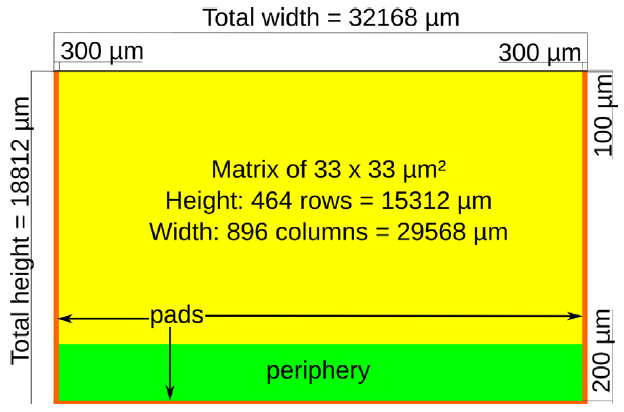
\includegraphics[scale=.7]{obelix_schematic}
\caption{OBELIX chip design.}
\label{fig:obelix_scheme}
\end{figure}

Moreover the sensor thickness has to be below 100 $\mu$m to respect the material budget constraint of 0.2\% $X_{0}$ and as consequence the depleted sensitive region should be lower than 50 $\mu$m, perfectly in agreement with the available thickness of MAPS  technology. 
To deal with the target hit rate of 120 MHz/$cm^{2}$, the timestamp clock signal can reach down to 25 ns, even if studies have demonstrated that a window of 100 ns (\textit{integration time}) is enough to limit to 320 Mbps the data throughput at the same expected hit rate. 
All characteristics inspected above allow to realize a sensor with high granularity in both space and time.\\

With respect to TJ-Monopix 2, which is equipped with a triggerless column-drain readout without memory at the periphery, OBELIX must have a triggered readout architecture, in order to satisfy the needs of Belle II. Moreover the latency is fixed to 5 (10) $\mu$s and it might operate up to 30 KHz trigger rate.

Single Event Upset~\autoref{foo:SEU} is a concern for the operation of the future detector but its size has not yet been quantified. Therefore an important feature of the chip must be to ensure that the control system is able to reset the sensor registers to default operational values at least every minutes. The reset frequency will be chosen after the measurement of the SEU cross section with OBELIX and the comparison to the occurence distribution of large energy loss in the experiment.

The expected power consumption instead, is expected to be about 200 mW$cm^{-2}$, a value which should allow air-cooling for the small areas corresponding to the two inner layers and liquid coolant for the outer ones. 

Its main design features are summarised in~\autoref{tab:obelix_features}.


\begin{table}[h!]
\centering
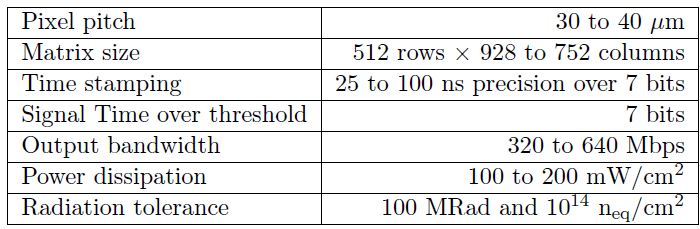
\includegraphics[scale=.7]{obelix_features}
\caption{Designed features of the OBELIX sensor.}
\label{tab:obelix_features}
\end{table}



\subsection{Sensor implementation}

As mentioned above, this new sensor is the development of TJ-Monopix 2, whose characteristics fit already the Belle II requirements (\autoref{tab:obelix_specification}).\\

\begin{table}[h!]
\centering
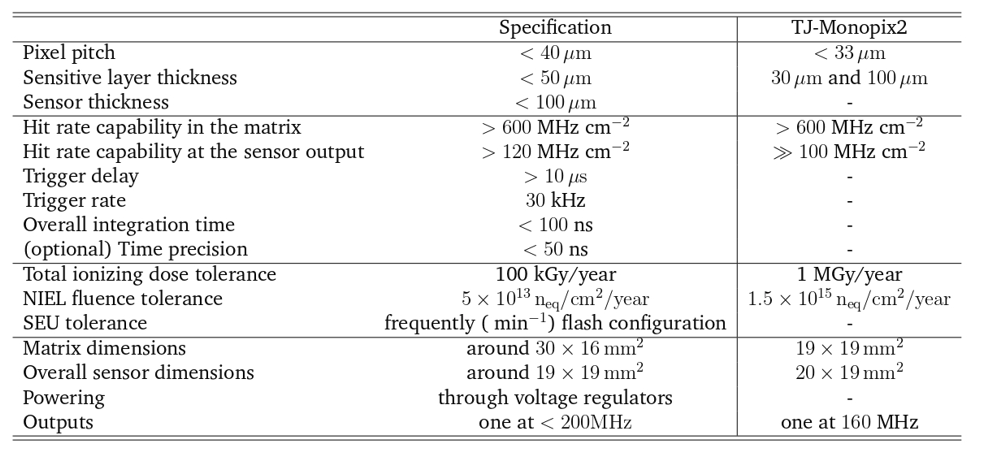
\includegraphics[scale=.6]{obelix_specification}
\caption{Comparison between OBELIX requirements and TJ-Monopix 2 features.}
\label{tab:obelix_specification}
\end{table}

From TJ-Monopix 2 design, the pixel size of \numproduct{33 x 33} $\mu m^{2}$ is maintained, as well as the layout of both digital and analogue parts (REFERENCE TO FOURTH). Also the Time-Over-Threshold method to digitize the signal is preserved, with a bus width of 7 bit, togheter with the column-drain readout architecture implemented for pairs of columns. Other features, which will be explained in depth in~\autoref{ch:TJ2}, have been conserved in the new design like the 3-bit register dedicated to the threshold tuning, but with a larger range of correction for the last bit. 
Moreover to aim at the integration time of 100 ns, the clock frequency which defines the precision of ToT and BCID (that is the timestamp), has been decreased from 40 to 20 MHz. So the current baseline for OBELIX timestamp precision is 50 ns.

Additionally two new modules have been added to the implementation, related to the Belle II trigger: the Trigger Logic Unit (TRU) and the Track Trigger Transmitter (TTT). 

\begin{description}
\item \textbf{Trigger Logic Unit (TRU)}
\end{description}

The TRU has the task to select the fired pixel information from the matrix which are in-time with the triggers sent by the Belle II system. In more details, this module employs two stages of memory in order to manage the data coming from the pixel matrix (\autoref{fig:obelix_tru}). These components are design in order to minimize power dissipation and to optimize the efficiency even in severe operating conditions: maximum hit rate of 120 MHz$cm^{-2}$, 30 KHz of trigger rate and 10 $\mu$s of trigger delay.

\begin{figure}[h!]
\centering
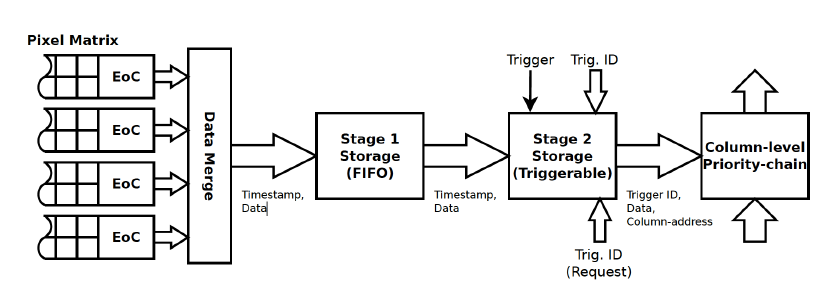
\includegraphics[scale=.8]{obelix_tru}
\caption{Schematic of the Trigger Logic Unit.}
\label{fig:obelix_tru}
\end{figure}

The first stage has to store the pixel information during the trigger delay. The second memory instead, has the function to compare the BCID of the fired pixel with each trigger time information buffered in a dedicated global memory which keeps track of received triggers. When they have a match, the pixel data is transferred to the Transmission Unit (TXU). In this way, the physics hits associated to a trigger but timestamped with a later BCID, for example due to timewalk effect, are also considered for further analysis.
Considering the BCID precision time, the time integration of the OBELIX sensor becomes 100 ns.


\begin{description}
\item \textbf{Track Trigger Transmitter (TTT)}
\end{description}

The TTT module divides the matrix in 8 logic regions (this value is still under study) and generates a one-byte word depending on the region that is fired. It is expected taht this information could be transmitted to trigger system within 100 ns and along a line of transmission parallel to the main data output of the sensor. 
This component behaviour is still under study and it needs of further simulations in correlation with the whole VTX system.


\begin{description}
\item \textbf{Control Unit (CRU) and power dissipation}
\end{description}

The OBELIX sensor, as well as TJ-Monopix 2, is configured by several registers which allow to set important features for its operation like threshold settings, masked pixels, time response of the pixels, but they also define its power consumption. The Control Unit is responsible for receiving these instructions about the configuration and the trigger information and at the same time sending out data coming from TXU module.

For what concern power dissipation, there are three main features which have the greatest impact: the biasing current flowing into the in-pixel amplifier (\textit{$I_{BIAS}$}), the BCID clock frequency (on which depends the timestamping precision) and the hit rate. In~\autoref{fig:obelix_power_cons} is shown the estimations of power dissipation as these parameters vary.


\begin{figure}[h!]
\centering
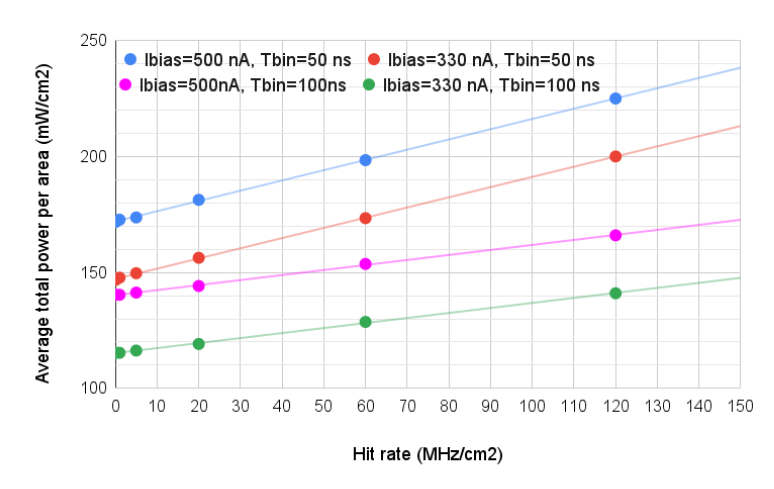
\includegraphics[scale=.8]{obelix_power_cons}
\caption{OBELIX sensor power dissipation depending on the front edn current (\textbf{$I_{bias}$}, the BCID frequency (\textbf{tbin}) and the hit rate).}
\label{fig:obelix_power_cons}
\end{figure}

As we can see, the power consumption at the maximum hit rate of 120 MHz$cm^{-2}$ exceeds by little more than 10\% the power budget of 200 mW$cm^{-2}$, considering the higher precision for the timestamp of 50 ns. Therefore to stay within the power budget it is necessary to find a compromise: reducing timing precision by worsening the BCID precision to 100 ns or decreasing the pre-amplifier biasing current causing a degradation of the time walk.


The first version of the sensor, called OBELIX-1, is being designed and the submission for fabrication is planned in the last month of 2023. A second improved version, OBELIX-2, will be designed based on performance studies on the first version and it is expected that it will be the final sensor needed for the experiment.\\

\bigskip

In this chapter we have introduced some of the fundamental aspects of the proposed VTX upgrade, suppported by continuous studies and simulations. In the following we will see in more details the technology on which the whole proposal is based: the CMOS Monolithic Active Pixel Sensor.





% --------------------------------------------
%		CAPITOLO 5
%---------------------------------------------
%% --------------------------------------------
%		CAPITOLO 5
%---------------------------------------------

\chapter{TJ-Monopix 2 characterization ??}
%\addcontentsline{toc}{chapter}{Caratterizzazione di TJ-Monopix 2}

\section{Matrix and flavors}

\subsection{Mask (operation) and noisy pixels}

\subsection{Analog and digital readout}

\subsubsection{BCID reset}
\begin{comment}
REFERENZE
\end{comment}

\subsubsection{Main registers (and conversion?)}



\subsection{Comparison of trends from data with simulation}
%\addcontentsline{toc}{subsection}{Confronto degli andamenti con le simulazioni}

To understand how the threshold's value changes with the settings of the chip, we take different measurements varying the values of the main registers which are responsible for it.
The results are compared with simultion done by Hung Pham (...).

\subsubsection{$I_{CASN}$}

This current is responsible of the output baseline. In a few words, higher this value, higher the baseline, lower the threshold and also a little bit the gain.

In figure \vref{fig:icasn_sim}, we can see the behaviour of the threshold and the gain, increasing the value o $I_{CASN}$.

\begin{figure}
\centering
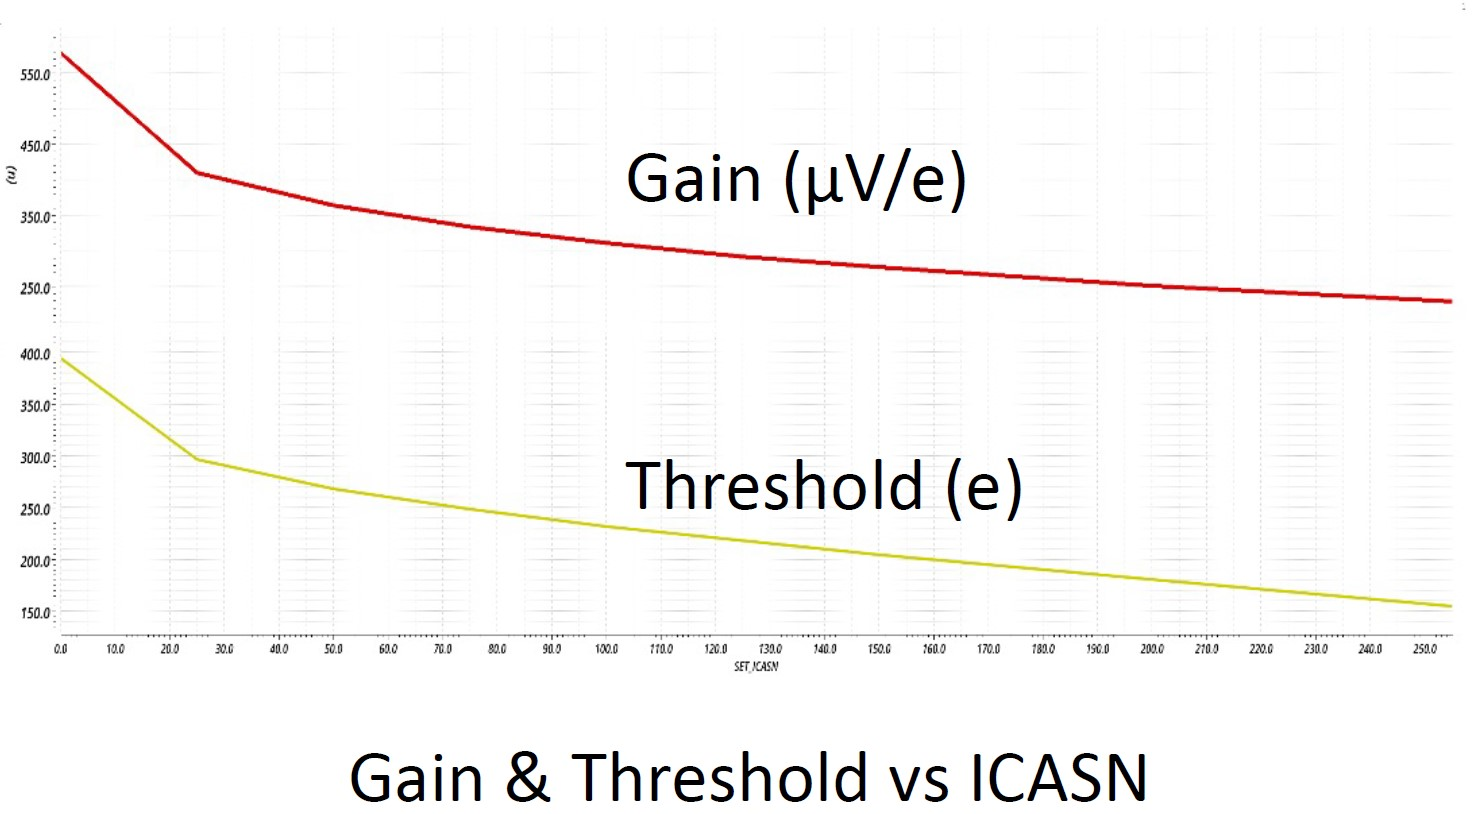
\includegraphics[scale=.5]{icasn_simulation}
\caption{Trends of Gain and Threshold increasing $I_{CASN}$.}
\label{fig:icasn_sim}
\end{figure}

To verify this behaviour, we run three different analysis (measurements) by fixing $I_{THR}$ = 20, 40, 64 and changing $I_{CASN}$ from 0  to 30 DAC, with a step of 5 DAC. We have done this enabling 200 pixels in the Cascode FE (rows: 472 - 512, cols: 225 - 230).

For each measurements we fit the threshold distribution with a gaussian function in order to obtain average values of the threshold and its dispersion.

\begin{itemize}
\item[$I_{THR}=64$]:

\begin{tabular}{c | c | c}
$I_{CASN}$ [DAC] & THR [DAC] & THR Dispersion [DAC]\\
\hline
0 & 61.43 & 2.45\\
5 & 53.42 & 2.45\\
10 & 50.33 & 2.45\\
15 & 48.21 & 2.41\\
20 & 46.70 & 2.38\\
25 & 45.49 & 2.52\\
30 & 46.09 & 2.50
\end{tabular}

\item[$I_{THR}=40$]:

\begin{tabular}{c | c | c}
$I_{CASN}$ [DAC] & THR [DAC] & THR Dispersion [DAC]\\
\hline
0 & 47.28 & 2.12\\
5 & 41.07 & 2.02\\
10 & 38.39 & 2.03\\
15 & 36.65 & 1.95\\
20 & 35.53 & 1.91\\
25 & NaN & NaN\\
30 & 33.37 & 2.04
\end{tabular}

Here we can see a particular setting, that is $I_{THR}=40$ AND $I_{CASN}$=25, for which the chip doesn't seem to work.

PIXEL THAT FIRE UP??

\item[$I_{THR}=20$]:

\begin{tabular}{c | c | c}
$I_{CASN}$ [DAC] & THR [DAC] & THR Dispersion [DAC]\\
\hline
0 & 34.43 & 1.95\\
5 & 28.10& 1.72\\
10 & 26.59 & 1.75\\
15 & 24.66 & 1.77\\
\end{tabular}
\medskip\\

\end{itemize}

In figure \vref{fig:alltrends_icasn} all trends obtained from these data are reported.

TREND OF DISPERSION?

\begin{figure}[h!]
\centering
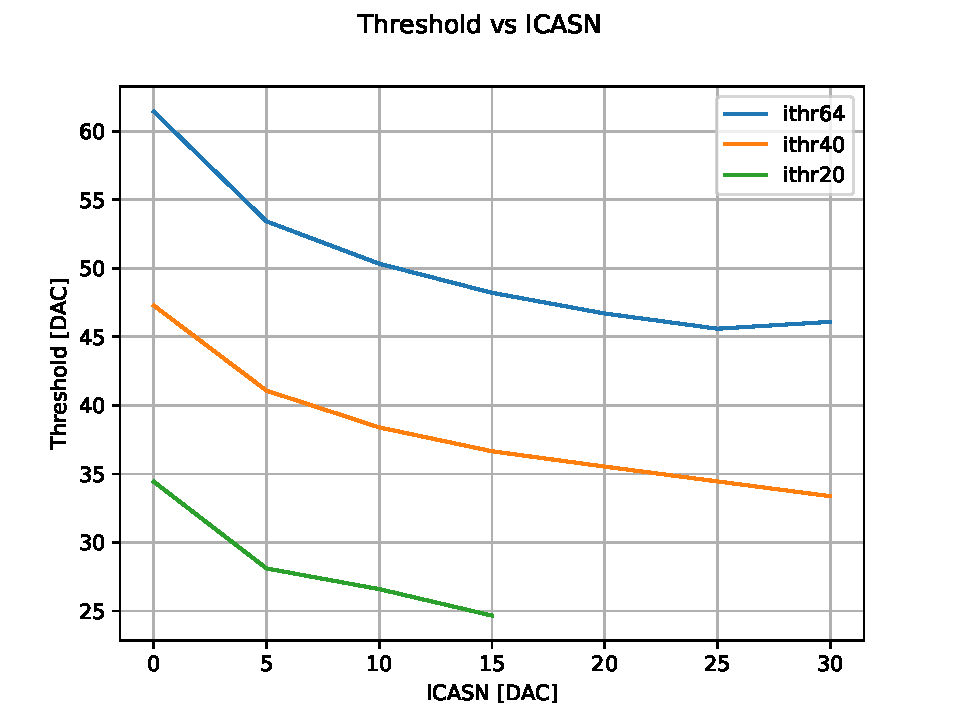
\includegraphics[scale=.7]{all_trends(ICASN)}
\caption{Threshold vs. $I_{CASN}$ for $I_{THR}$= 20, 40, 64.}
\label{fig:alltrends_icasn}
\end{figure}

\subsubsection{$I_{THR}$}

Reusing the same data of the previous measurements, we can also study the trend of the threshold changing the value of $I_{THR}$ and fixing that of $I_{CASN}$. We consider only $I_{CASN}$ from 0 to 15 DAC, because for highr values we don't have enough values of the threshold (only two, for $I_{THR}$=40, 64). The results are showed in figure \vref{fig:alltrends_ithr}.

\begin{figure}[h!]
\centering
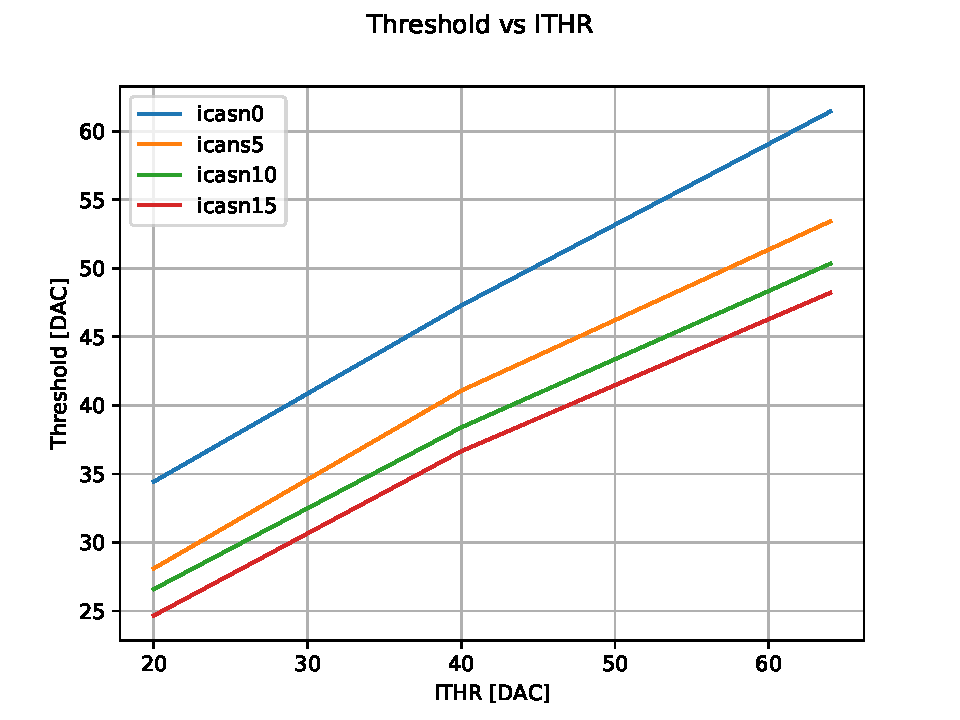
\includegraphics[scale=.7]{all_trends(ITHR)}
\caption{Threshold vs. $I_{THR}$ for $I_{CASN}$= 0, 5, 10, 15.}
\label{fig:alltrends_ithr}
\end{figure}

We can compare them with the simulation done by Hung Pham (\vref{fig:ithr_sim}). 

\begin{figure}[h!]
\centering
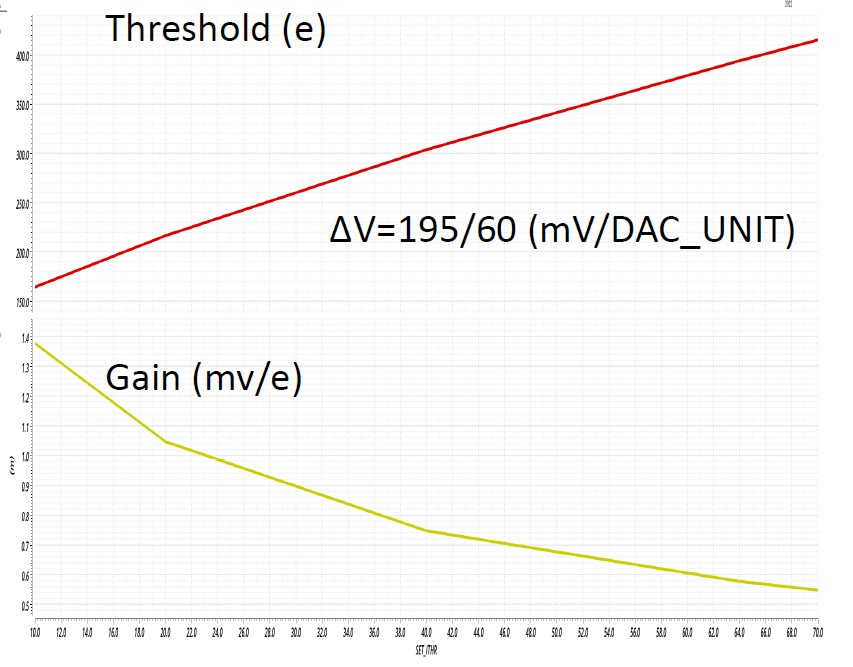
\includegraphics[scale=.7]{ithr_simulation}
\caption{Trends of Gain and Threshold increasing $I_{CASN}$.}
\label{fig:ithr_sim}
\end{figure}

\subsubsection{Time over Threshold (ToT)}

The last analysis that we have done to make a comparison with the simulations, is about the trend of the ToT, changing the value of $I_{CASN}$ for a fixed value of $I_{THR}$ and vice versa. In particular we consider the data obtained with $I_{CASN}$ fixed to 0 DAC and $I_{THR}$ to 64 DAC, which are the values for this registers, studied and used during the Test Beam in Desy.

\begin{figure}[h!]
\centering
\subfigure[ToT vs $I_{THR}$ ($I_{CASN}$=0 DAC) - Data]
{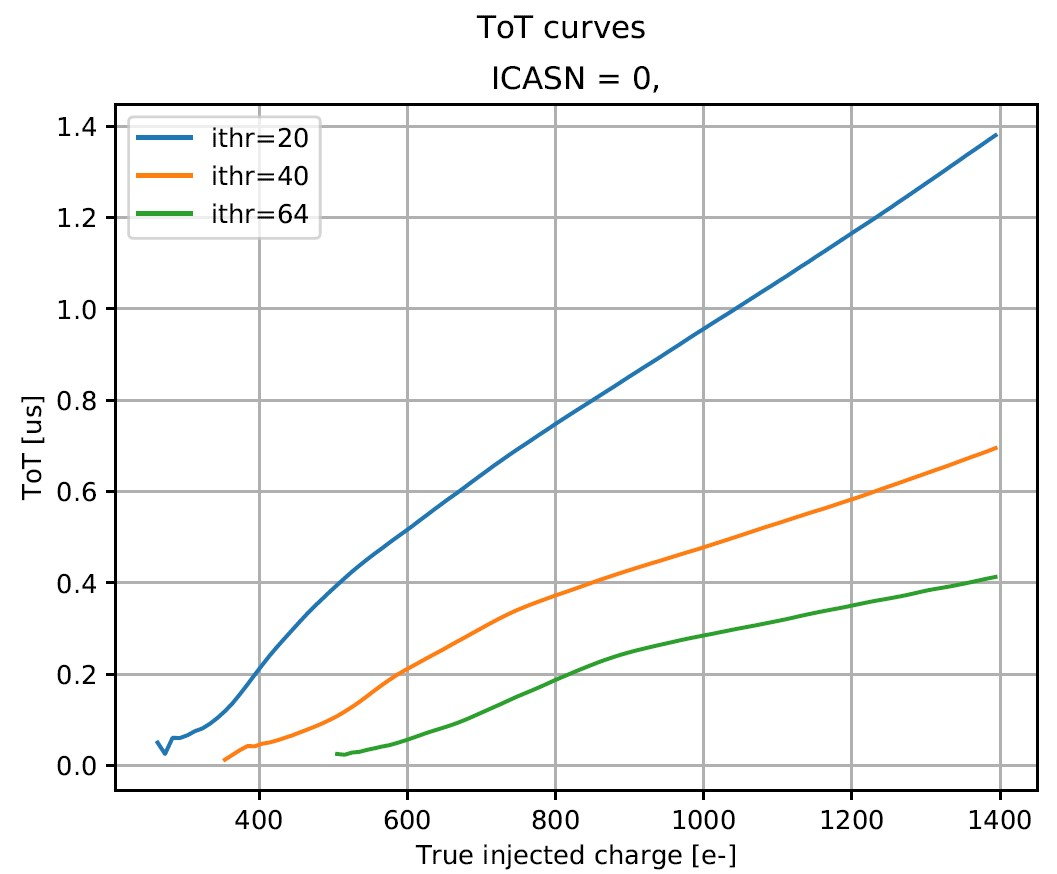
\includegraphics[scale=0.5]{tot_curves_icasn0}}\quad
\subfigure[ToT vs $I_{THR}$ ($I_{CASN}$=0 DAC) - Simulation]
{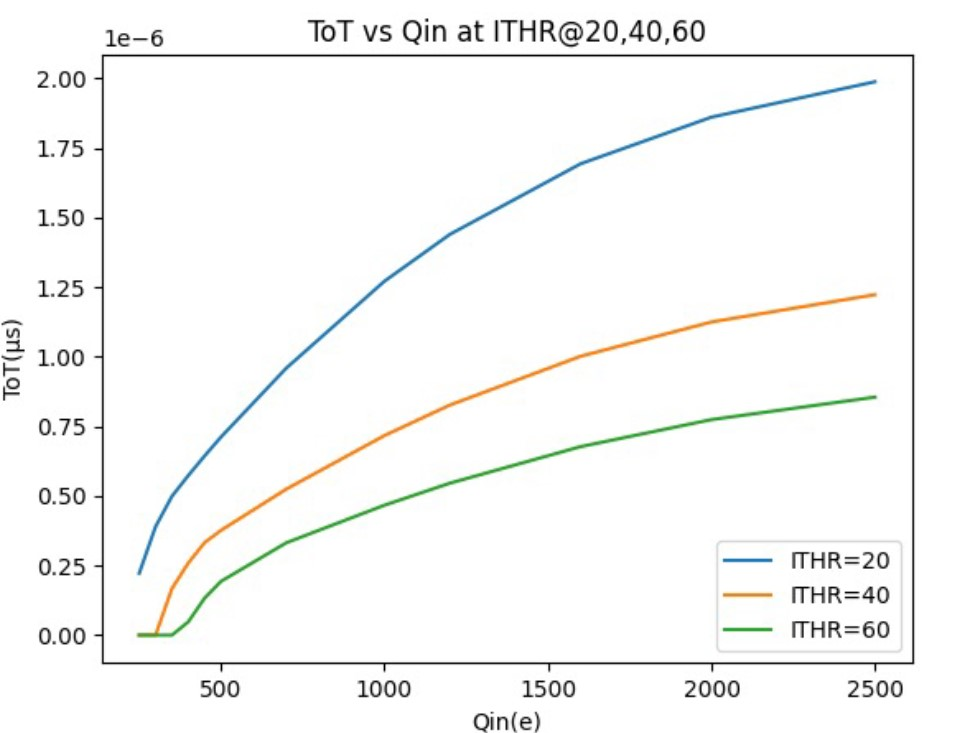
\includegraphics[scale=0.4]{tot_curves_icasn0_simu}}\\
\caption{.}
\label{fig:tot_vs_ithr}
\end{figure}

\begin{figure}[h!]
\centering
\subfigure[ToT vs $I_{CASN}$ ($I_{THR}$=64 DAC) - Data]
{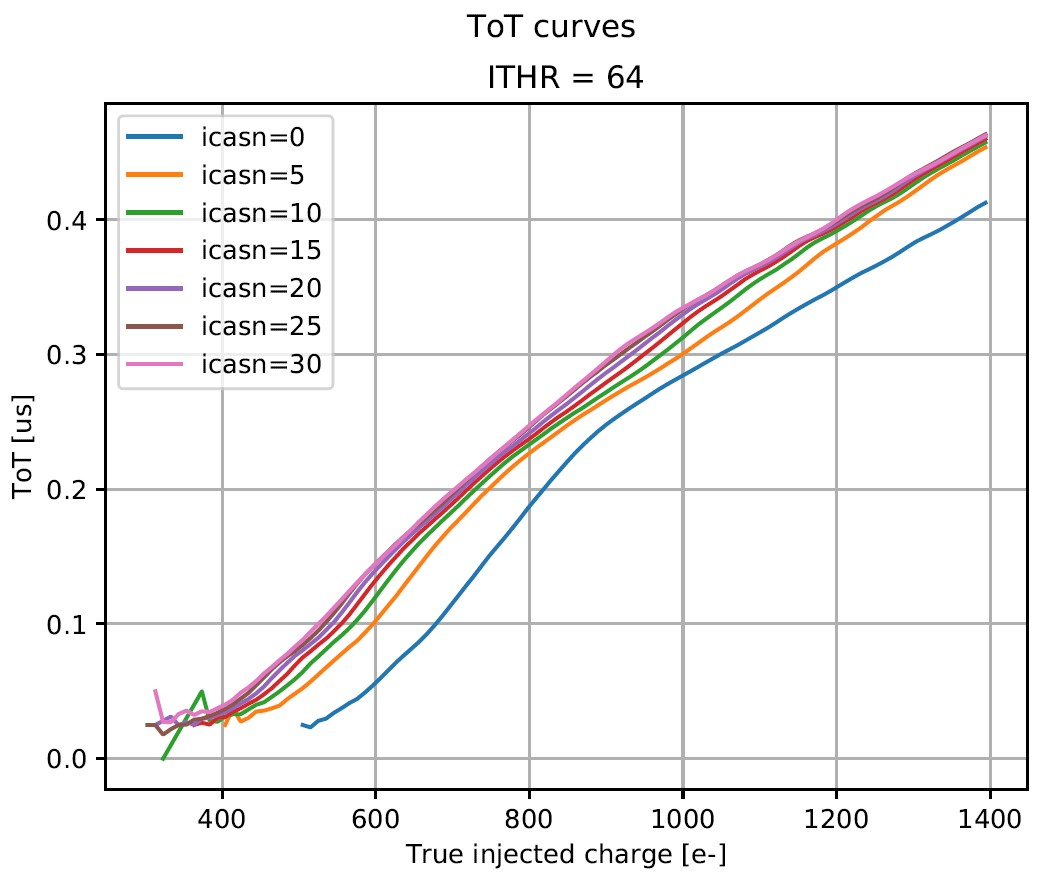
\includegraphics[scale=0.5]{tot_curves_ithr64}}\quad
\subfigure[ToT vs $I_{CASN}$ ($I_{THR}$=64 DAC) - Simulation]
{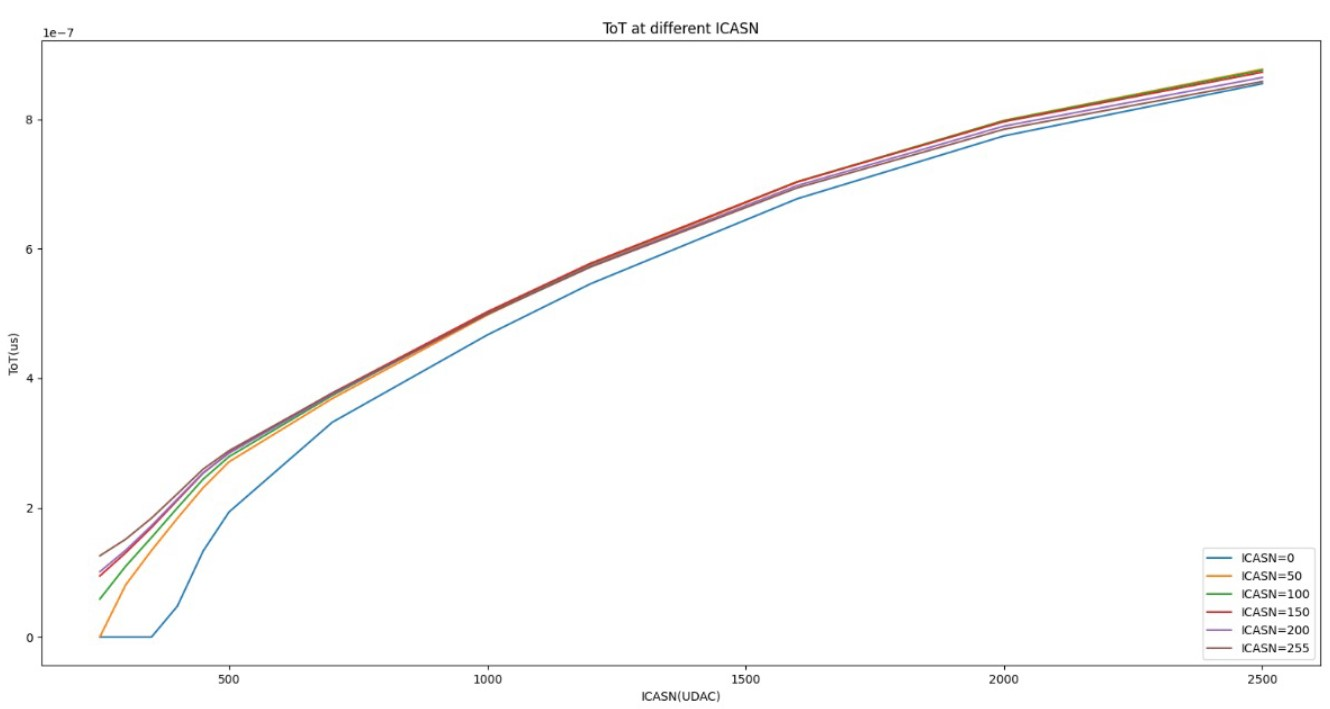
\includegraphics[scale=0.4]{tot_curves_ithr64_simu}}\\
\caption{.}
\label{fig:tot_vs_icasn}
\end{figure}

\section{Characterization by injection}
%\addcontentsline{toc}{section}{Caratterizzazione tramite l'iniezione}

In the prototype under test (study), W14R12 chip, some problems (raised up) arose right from the beginning, linked (concerned) pixels of the matrix both for the analog and digital part.
Despite its predecessor Tj-Monopix 1, Tj-Monopix 2 is equipped with a circuit which allows the \textit{threshold tuning}.In other words it can adjust, even if only few DAC, every pixel threshold, in order to have a global threshold on the matrix as uniform as possible, or in any case a dispersion as small as possible.

Preliminarly it's necessary to study the threshold distribution on the whole matrix. We have separately analyzed the four flavors, to be able to study their main difference in working (performance) and features.

The ultimate purpose of this measurement is to describe (depict, mark out) the behaviour of each pixel, injecting a charge equivalent to the typical energy released from electrons emitted in radioactive decays (decays of radioactive materials) and in particular those produced by the electronic capture of \ch{^{55}Fe} (presente in laboratorio). As explained in the previous section (reference), the \ch{^{55}Fe} has an emission spectrum (lines) with lines quite peaked (sharp) and this allows to compare data more easily. The first line is at 5.9 KeV which corresponds on average to about 1616 $e^{-}$ released (through the pixel??).
For this reason during the injection measurement, it's mandatory to know the conversion between DAC and $e^{-}$ (reference) and to inject charges in order to study pixel behaviour  the right region, which are more interesting from a physical point of view.

\begin{figure}[h!]
\centering
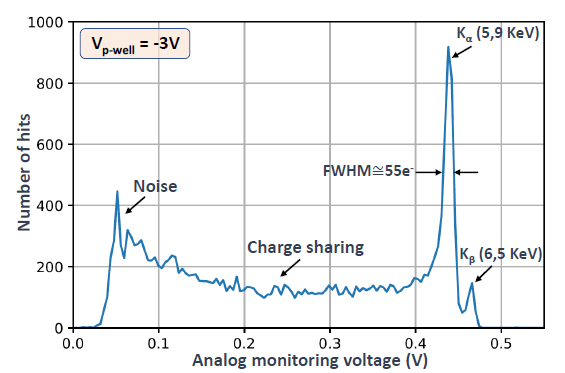
\includegraphics[scale=0.8]{spectrum_fe}
\caption{\ch{^{55}Fe} (radiactive source) emission spectrum using the analog output of a PMOS reset front-end of TJ-Monopix 1. (referenceeeeee)}
\label{fig:fespectrum}
\end{figure}

%------------------------------------------------------------
\subsection{Injection circuit issues}

In carrying out the measurements mentioned above, we noticed (NO) some issues with the injection circuit which limits its working range: (as a matter of fact) the height of the injection pulse is expected to grow (increase) linearly up to a value of (about) $\approx$ 140 DAC, but  above this (quantity) value, the circuit increases not only a little the height of the signal, but also the threshold artificially grows by a certain amount of $\Delta V$ (or equivalently of $\Delta Q$, related by the conversion factor....REFERENCE).
Moreover, for injection height grater than 200 DAC, only the threshold grows, without increasing the actual injected charge in any way.

For this reason, the investigation on the (values) behaviour of the threshold and its dispersion of all flavours of the matrix, required a series of additional measurements.

%-------------------------------------------------------
\subsection{Measurement of the average shift of the threshold value for injected charge greater than 140 DAC}

To evaluate this artificial shift of the threshold, two different measurements of the threshold and its dispersion have been done, for each flavor:

\begin{itemize}
\item for an injected charge equal to 140 DAC $\rightarrow$ before the saturation region;
\item for an injected charge equal to 200 DAC $\rightarrow$ almost the maximum limit of the saturation region (from this value onward only the threshold increases, not the injected charge).
\end{itemize}

The threshold distributions obtained from each measurements have been fitted to extract an average value on the whole flavor. Naming $Q_{th, 140}$ and $Q_{th, 200}$  the threshold obtained from injections of 140 and 200 DAC respectively, the mean shift has been estimated by:

\begin{equation}
\Delta Q = Q_{th,200} - Q_{th,140}
\end{equation}

Eventually, this charge shift has been subtracted from data collected for injection pulses of 200 DAC, in order to extrapolate (deduce) the behaviour of the injected pixels up to a value fo 170 DAC.

What has been obtained for each flavor is reported in the following section, together with a briefly explanation of the method used to estimate (evaluate) the threshold.


%--------------------------------------------------------------------
\subsection{Threshold and S-Curve}
%\addcontentsline{toc}{subsection}{Curva S e threshold}

In order to obtain the thresold value for every pixel, each one has to be injected a random (arbitrary) number of times (we have chosen 100 times) for each value of the injection pulse between a minimum value, chosen set the chip register ''\textbf{VL}'' and a maximum value, set by the ''\textbf{VH}'' register, with a random step which is 1 for us.(ANCHE NO)

So with(fixed) the value of the injection pulse fixed, the mean of 100 output are considered. In this way, the typical curve, better known as ''\textit{S-curve}'', is obtained for each pixel. It is an \textit{error-function} from which the value of the threshold is evaluated considering (taing, extractin, pulling out) the value of the injected charge at half of the curve's maximum height.

Plotting the number of hits observed on each pixel divided by the total number of injections, for each injected charge, the half height corresponds to a charge value for which the pixel detects 50 hits of 100 injected and so when it has an occupancy of 0.5.

%%%%SPIEGARE METODO DI LUDOVICO???? 


%%%METTI ESEMPIO S-CURVE
\begin{comment}
\begin{figure}
\centering
\includegraphics[]{}
\caption{An example of the S-Curve and the evluation of the threshold.}
\label{ex_scurve}
\end{figure}
\end{comment}

In the following are reported the results of this study for the flavors of all matrix.

\subsubsection{Normal FE}

As epxplained in the section (reference) the first flavor of the matrix is the \textbf{Normal FE}, which consist of 512 rows (0-511 in registers?) and 224 columns for a total of 114.688 pixels. In figure \vref{fig:norm_scurve_140} are plotted all the s-curves of the Normal flavor pixels. The chip registers have been set with the same values used during the Test Beam at Desy (during...) which are reported in table \vref{tab:tb_settings}.

%%%COLORAAAAAAAA
COLORAAAAA

\begin{table}[h!]
\centering
\begin{tabular}{c|c}
Registri & Default Settings (''GOE'') \\
\hline
ITHR & 64 \\
\hline
IBIAS & 50 \\
\hline
VRESET & 143 \\
\hline
ICASN & 0 \\
\hline
VCASP & 93 \\
\hline
VCASC & 228 \\
\hline
IDB & 100 \\
\hline
ITUNE & 53 \\
\hline
VCLIP & 255 \\
\hline
ICOMP & 80 \\
\hline
IDEL & 88 \\
\hline
IRAM & 50 \\
\hline
\end{tabular}
\caption{Settings of the main registers used for the W14R12 chip, for Normale and Cascode flavors, during the Test Beam in Desy.}
\label{tab:tb_settings}
\end{table}

\begin{figure}[h!]
\centering
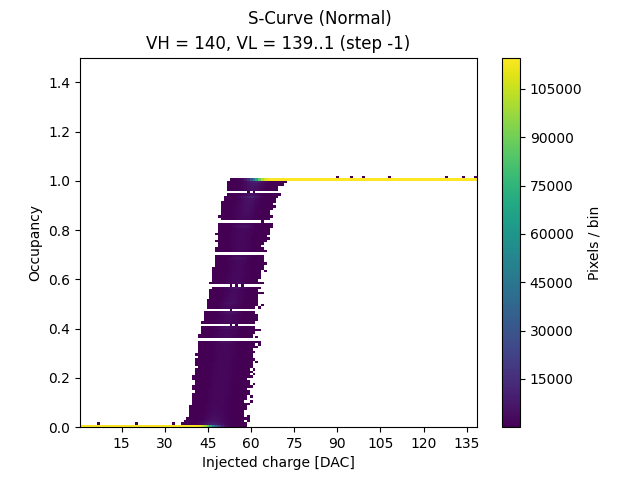
\includegraphics[scale=.6]{all_norm_thscan_140}
\caption{S-curves of all pixels of the Normal FE with an injection pulse of 140 DAC.}
\label{fig:norm_scurve_140}
\end{figure}

Using this setting, none of the pixels were noisy and so it wasn't necessary introduce (use, ...) any mask.

As already explained in the previous section (reference?) the threshold distributions from the two different measurements with an injection pulse of 140 and 200 DAC respectively, have been fitted and they are showed in figure \vref{fig:thdist_norm}

\begin{figure}[h!]
\centering
\subfigure[VH = 140 DAC]
{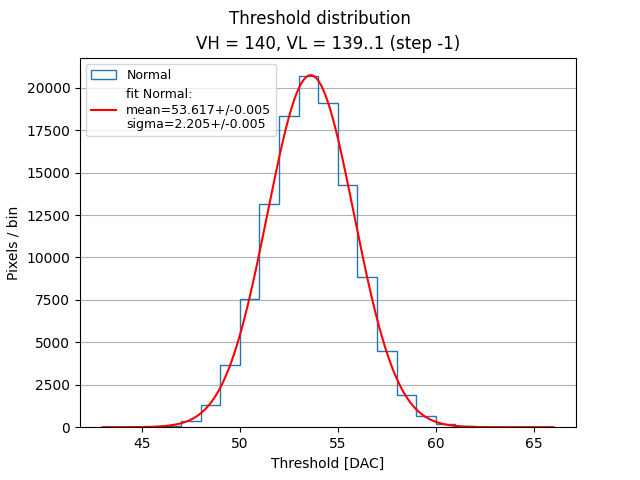
\includegraphics[scale=0.6]{all_norm_thdist_140}}\quad
\subfigure[VH = 200 DAC]
{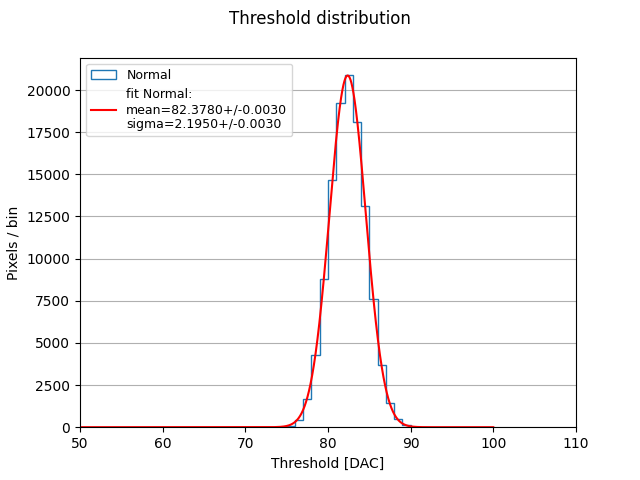
\includegraphics[scale=0.6]{all_norm_thdist_200}}\\
\caption{Threshold distributions of \textbf{Normal} flavor before and at the maximum saturation, respectively.}
\label{fig:thdist_norm}
\end{figure}
 
For the greater (higher) injection height, 8 different measurement have be actually done, each one on 28 consecutive columns and on all rows. Then data have been put together to obtain a single (summary) plot on the whole flavor. Same procedure has been preformed on the \textbf{Cascode FE}.


\subsubsection{Cascode FE}

\textbf{Cascode FE} is the second flavor and like \textbf{Normal FE} it consists of 512 rows (0-511) and 224 columns (224-447) for a number of total pixels equal to 114.688. Also for this study (measurement) the same values' registers of the setting used during the Test Beam in Desy (table \vref{tab:tb_settings}) have been used and there weren't find noisy pixels. 
In figure \vref{fig:casc_curve_140} the S-curves of all pixels ar showed.

\begin{figure}[h!]
\centering
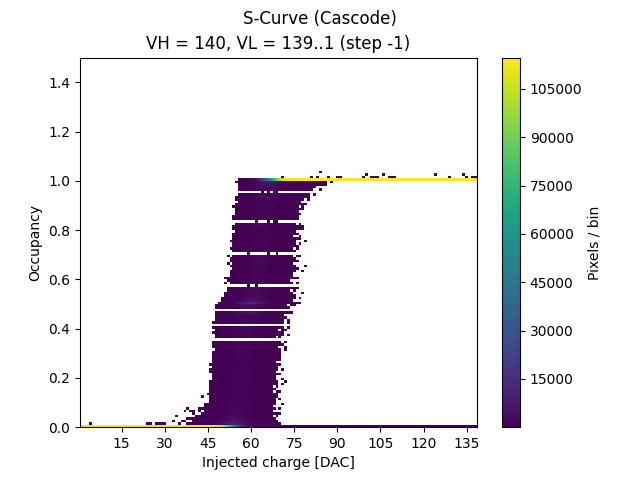
\includegraphics[scale=.6]{all_casc_thscan_140}
\caption{S-curves of all pixels in the \textbf{Cascode} flavor with an injection pulse of 140 DAC.}
\label{fig:casc_scurve_140}
\end{figure}

The fit of the threshold distributions instead, are showed in figure \vref{fig:thdist_casc}.

\begin{figure}[h!]
\centering
\subfigure[VH = 140 DAC]
{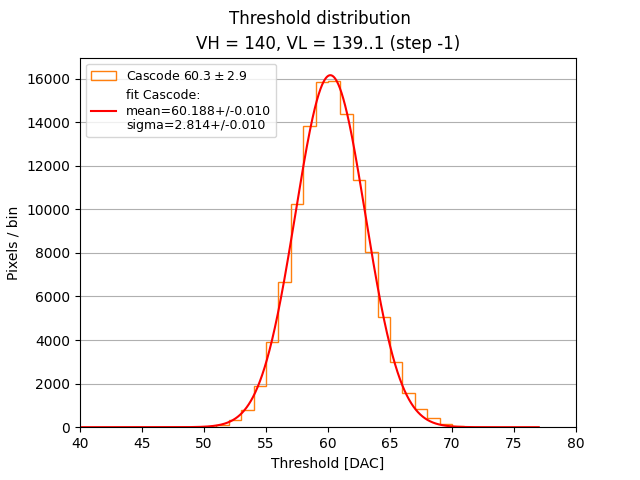
\includegraphics[scale=0.6]{all_casc_thdist_140}}\quad
\subfigure[VH = 200 DAC]
{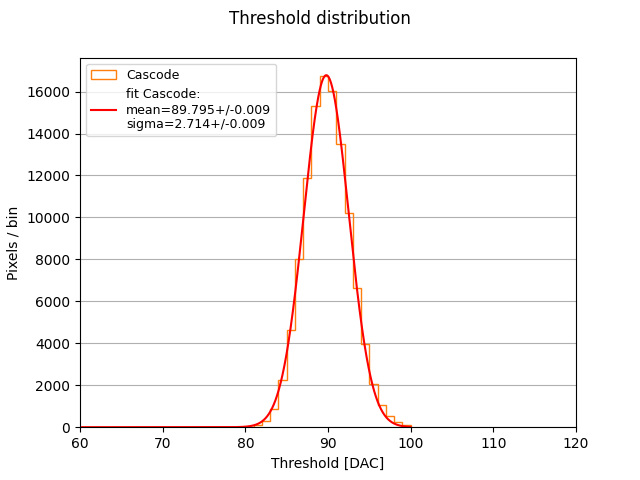
\includegraphics[scale=0.6]{all_casc_thdist_200}}\\
\caption{Threshold distributions of \textbf{Cascode} flavor before and at the maximum saturation, respectively.}
\label{fig:thdist_casc}
\end{figure}


\subsubsection{HV-Cascode FE}

The third flavor is \textbf{HV-Cascode FE} where HV stands for \textbf{High Voltage} and it is formed (consists) of 512 rows (0-511) and 32 columns (448-479) for a total number of pixel equal to 16384. Also for these last two flavors, the main chip registers are set with the same values tested and used during the Test Beam (@Desy). They are reported in table \vref{tab:tb_hv_settings}.

\begin{table}[h!]
\centering
\begin{tabular}{c|c}
Registri & Default Settings (''GOE'') \\
\hline
ITHR & 30 \\
\hline
IBIAS & 60 \\
\hline
VRESET & 100 \\
\hline
ICASN & 8 \\
\hline
VCASP & 40 \\
\hline
VCASC & 228 \\
\hline
IDB & 100 \\
\hline
ITUNE & 53 \\
\hline
VCLIP & 255 \\
\hline
ICOMP & 80 \\
\hline
IDEL & 88 \\
\hline
IRAM & 50 \\
\hline
\end{tabular}
\caption{Settings of the main registers used for the W14R12 chip, for the HV's flavors, during the Test Beam in Desy.}
\label{tab:tb_hv_settings}
\end{table}

As we can see from the plot of the alle S-curves in figure \vref{fig:hvc_scurve_140}, with these choices of values' registers, there were a lot of noisy pixels, but at this stage of measurements, they were not masked.

\begin{figure}[h!]
\centering
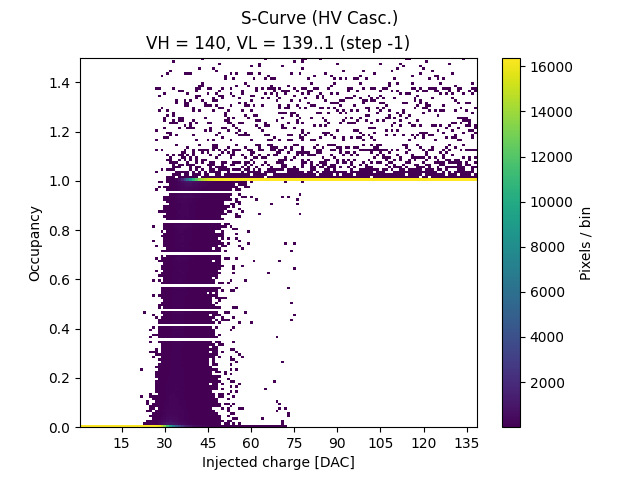
\includegraphics[scale=.6]{all_HVc_thscan_140}
\caption{S-curves of all pixels in \textbf{HV Cascode} flavor with an injection pulse of 140 DAC.}
\label{fig:hvc_scurve_140}
\end{figure}

In figure \vref{fig:thdist_hvc} are showed the fit of the threshold distributions for the two different injections pulse.

\begin{figure}[h!]
\centering
\subfigure[VH = 140 DAC]
{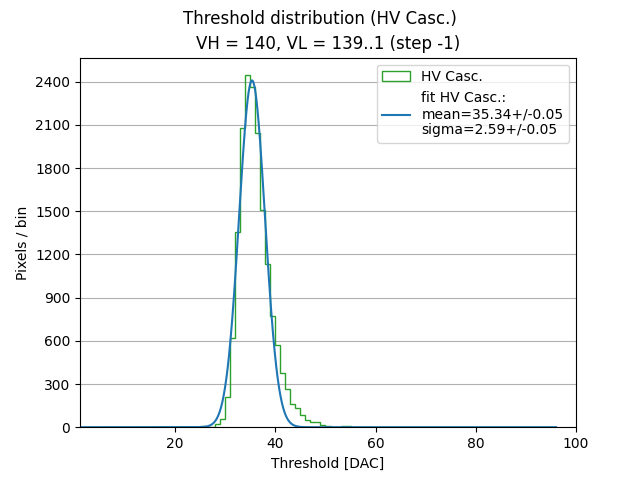
\includegraphics[scale=0.6]{all_HVc_thdist_140}}\quad
\subfigure[VH = 200 DAC]
{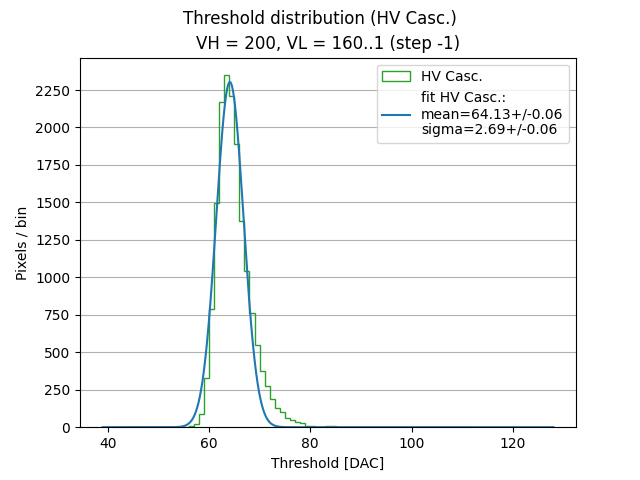
\includegraphics[scale=0.6]{all_HVc_thdist_200}}\\
\caption{Threshold distributions of \textbf{HV Cascode} flavor before and at the maximum saturation, respectively.}
\label{fig:thdist_hvc}
\end{figure}


\subsubsection{HV-Normal FE}

The fourth and last flavor is the \textbf{HV-Normal FE} which consists of 512 rows (0-511) and 32 columns (479-511) for a total number of pixel equal to 16.384. The main registers have been set with the values reported in table \vref{tab:tb_hv_settings}.
In figure \vref{fig:hv_scurve_140}, the S-curves of all pixel in the flavor. Also here we can see that there were some noisy pixels unmasked.
Moreover, in this final flavor, the last 16 columns were not working and as a matter of fact they had return a peak of threshold near the value 0, which is excluded from the threshold distributions plots.

So actually in this part of the matrix, the real number of pixel studied was the half of the total, such as 8192 pixels.



\begin{figure}[h!]
\centering
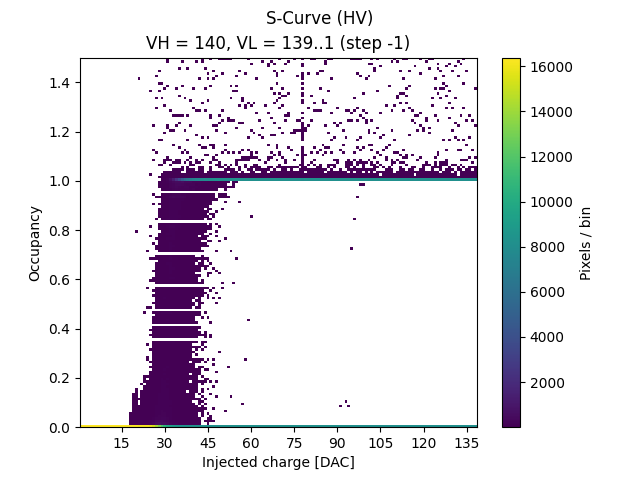
\includegraphics[scale=.6]{all_HV_thscan_140}
\caption{S-curves of all pixels in \textbf{HV Cascode FE} with an injection pulse of 140 DAC.}
\label{fig:hv_scurve_140}
\end{figure}

In figure \vref{fig:thdist_hvc} the fit of the threshold distributions for the two different values of injection height are reported.


\begin{figure}[h!]
\centering
\subfigure[VH = 140 DAC]
{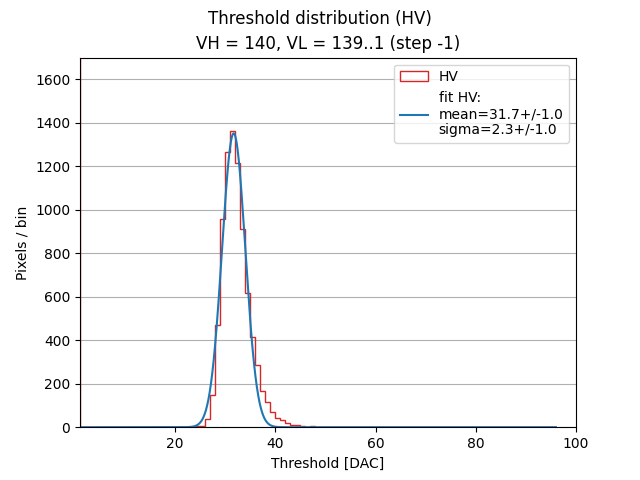
\includegraphics[scale=0.6]{all_HV_thdist_140}}\quad
\subfigure[VH = 200 DAC]
{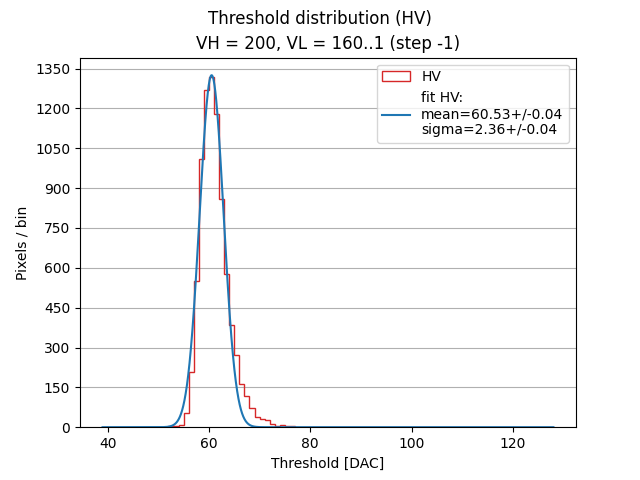
\includegraphics[scale=0.6]{all_HV_thdist_200}}\\
\caption{Threshold distributions of \textbf{HV} flavor before and at the maximum saturation, respectively.}
\label{fig:thdist_hvc}
\end{figure}



\subsection{Noise and Equivalent Noise Charge (ENC)}
%\addcontentsline{toc}{subsection}{Noise and Equivalent Noise Charge (ENC)}

\subsection{Curve del Time Over Threshold (TOT) e fit}
%\addcontentsline{toc}{subsection}{Curve del Time Over Threshold (TOT) e fit}

\section{Caratterizzazione con le sorgenti radioattive}
%\addcontentsline{toc}{section}{Caratterizzazione con le sorgenti radioattive}

Fe55, Am241, Cd109, Sr190

\subsection{Calibrazione della capacità di iniezione}
%\addcontentsline{toc}{subsection}{Calibrazione della capacità di iniezione}






%%%%%%%%%%%%%%%%%%%%%%%%%%
%			BIBLIOGRPAHY
%%%%%%%%%%%%%%%%%%%%%%%%%%

%1. THESIS MUSTAKAS




%%%%%%%%%%%%%%%%%%%%%%%%%%%%%%%%%%%%%%%%%

% --------------------------------------------
%		CONCLUSIONI 
%---------------------------------------------
\chapter{Conclusions}
%\addcontentsline{toc}{chapter}{Conclusioni}




% --------------------------------------------
%		INDICE 
%---------------------------------------------
%\index{Conclusioni}
%\index{Pixel ibridi}
%\index{Ibridizzazione}
\printindex

% --------------------------------------------
%		BIBLIOGRAFIA 
%---------------------------------------------

% --------------------------------------------
%		ACRONIMI
%---------------------------------------------

% --------------------------------------------
%		LIST OF FIGURE AND TABLES 
%---------------------------------------------

\end{document}